%                                                                 aa.dem
% AA vers. 9.1, LaTeX class for Astronomy & Astrophysics
% demonstration file
%                                                       (c) EDP Sciences
%-----------------------------------------------------------------------
%
% \documentclass[referee]{aa} % for a referee version
%\documentclass[onecolumn]{aa} % for a paper on 1 column  
%\documentclass[longauth]{aa} % for the long lists of affiliations 
%\documentclass[letter]{aa} % for the letters 
%\documentclass[bibyear]{aa} % if the references are not structured 
%                              according to the author-year natbib style

%

\documentclass{aa}  

%
\usepackage{graphicx}
\usepackage{amsmath,amsfonts,amssymb}
\usepackage{natbib}


%%%%%%%%%%%%%%%%%%%%%%%%%%%%%%%%%%%%%%%%
\usepackage{txfonts}
\usepackage{xcolor}

\usepackage{blindtext}
%%%%%%%%%%%%%%%%%%%%%%%%%%%%%%%%%%%%%%%%
% \usepackage[options]{hyperref}
% To add links in your PDF file, use the package "hyperref"
% with options according to your LaTeX or PDFLaTeX drivers.
\usepackage{float}
%\usepackage{stfloats}
\usepackage{dblfloatfix}
\usepackage{afterpage}
\usepackage{ifthen}
\usepackage[morefloats=12]{morefloats}

\usepackage{placeins}
\usepackage{multicol}
%\usepackage[breaklinks,colorlinks,citecolor=blue]{hyperref}
\bibpunct{(}{)}{;}{a}{}{,}
\usepackage[switch]{lineno}
\definecolor{linkcolor}{rgb}{0.6,0,0}
\definecolor{citecolor}{rgb}{0,0,0.75}
\definecolor{urlcolor}{rgb}{0.12,0.46,0.7}
\usepackage[breaklinks, colorlinks, urlcolor=urlcolor,
    linkcolor=linkcolor,citecolor=citecolor,pdfencoding=auto]{hyperref}
\hypersetup{linktocpage}
\usepackage{bold-extra}
\usepackage{tabularx, booktabs}

%Planck style file, to be used with A&A style to produce Planck papers for publication.
%
% version 28 September 2010 --- useful macros --- CRL
% version 17 October 2010   --- first cut at important instrument values, from Daniele Mennella and
%                               Francois Bouchet, 13 October 2010 --- CRL
% version 18 October 2010   --- LFI FWHM changed to one value per feed, rather than M & S separately
%                               LFI FWHM uncertainties added for individual feeds.  Corrections made
%                               to LFI values. --- Andrea Zacchei
% version 24 October 2010   --- added to and corrected definitions.  No changes made to instrument
%                               quantities. --- CRL 
% version 31 October 2010   --- added definition of \muKHz. --- CRL
%
% version 15 November 2010  --- fixed conflict with aa.cls in definition of \endtable
%                               by naming the command below "\endPlancktable".  See section
%                               13.16 of the Style Guide.
%
% version 06 December 2010  --- Set up names with and without units.
%                               Add \allearlypapers command to ensure that all early papers are
%                               included in the reference list.
%                               Define macro for the name of the 4He JT cooler.
%
% version 07 December 2010  --- removed extraneous "planck2011-1.2" entry in \allearlypapers
%
% version 12 December 2010  --- added \endPlancktablewide command to set tablenotes to the full
%                               page width in the \begin{table*}...\end{table*} environment when
%                               the ``twocolumn'' option is specified in the \documentclass command.
%                               (It would be more elegant to extract the appropriate width from the
%                               aa.cls system at the time of execution, but that is buried more
%                               deeply in the system than I investigated.)
%
% version 05 January 2011   --- added unit \MJysr.  HFI performance values updated per FRB email
%                               01/05/2011 02:38-0800, and Brendan Crill email 01/05/2011 18:08 -0800.
%
% version 06 January 2011   --- changed \scriptscriptstyle primes to \scriptstyle, to better match the
%                               tx fonts used by A&A.
%
% version 07 January 2011   --- modified \allearlypapers to correspond with final early paper list.  
%                               Fixed 545 GHz center frequency.
%
% version 07 January 2011b  --- changed LFI white-noise sensitivity numbers to correct problem with units
%
% version 05 July 2011      --- added \Msol and \Lsol to get the symbols for solar mass and luminosity.
%                               Deleted previous definitions of \solar and \sol, which were equivalent
%                               to the new \Msol.
%
% version 16 August 2011    --- changed comments on \endPlancktable and \endPlancktablewide for clarity
%
% version 11 September 2011 --- changed definition of \tablenote to make footnote labels italic, as per A\&A
%
% version 26 April 2011     --- changed definition of \Planck to agree with what is said in the Style Guide (!)
%
% version 04 Dec 2013       --- included 2013 results references
%
% version 17 Jan 2014       --- included fix to bibtex file v4.3, i.e. \providecommand{\sorthelp}[1]{}
%
% version 26 Jul 2014       --- fixed incompatibility problem with aa.cls v8.0 and v8.2.  v8.2 should now be used
%                               for all Planck papers.
%                           --- fixed problem in definition of "\all2013resultspapers" that introduced a blanck
%                               into the reference to p06b.
%                           --- removed all the parameter definition stuff at the end.  We weren't using it, and
%                               it took up a lot of space.
%
% version 28 Jan 2015       --- added "\alltwentyfiftennresultspapers" and corrected "\all2013resultspapers" to
%                               "\all20thirteenresultspapers",
%
% Usage:  after the \documentclass[traditabstract]{aa} command in the La\TeX\ input file,
%         add this command:      \input Planck.tex


\def\setsymbol#1#2{\expandafter\def\csname #1\endcsname{#2}}
\def\getsymbol#1{\csname #1\endcsname}

%-----------------------------------------------------------------------
% Planck
%-----------------------------------------------------------------------
\def\Planck{\textit{Planck}}

%-----------------------------------------------------------------------
% The Planck Helium-4 JT cooler
%-----------------------------------------------------------------------
\def\HeJT{$^4$He-JT}

%-----------------------------------------------------------------------
% To include all Planck Early Results papers in the reference lists
%-----------------------------------------------------------------------
\def\allearlypapers{\nocite{planck2011-1.1, planck2011-1.3, planck2011-1.4, planck2011-1.5, planck2011-1.6, planck2011-1.7, planck2011-1.10, planck2011-1.10sup, planck2011-5.1a, planck2011-5.1b, planck2011-5.2a, planck2011-5.2b, planck2011-5.2c, planck2011-6.1, planck2011-6.2, planck2011-6.3a, planck2011-6.4a, planck2011-6.4b, planck2011-6.6, planck2011-7.0, planck2011-7.2, planck2011-7.3, planck2011-7.7a, planck2011-7.7b, planck2011-7.12, planck2011-7.13}}

%-----------------------------------------------------------------------
% To include all Planck 2013 Results papers in the reference lists
%-----------------------------------------------------------------------
\def\alltwentythirteenresultspapers{\nocite{planck2013-p01, planck2013-p02, planck2013-p02a, planck2013-p02d, planck2013-p02b, planck2013-p03, planck2013-p03c, planck2013-p03f, planck2013-p03d, planck2013-p03e, planck2013-p01a, planck2013-p06, planck2013-p03a, planck2013-pip88, planck2013-p08, planck2013-p11, planck2013-p12, planck2013-p13, planck2013-p14, planck2013-p15, planck2013-p05b, planck2013-p17, planck2013-p09, planck2013-p09a, planck2013-p20, planck2013-p19, planck2013-pipaberration, planck2013-p05, planck2013-p05a, planck2013-pip56, planck2013-p06b, planck2013-p01a}}

%-----------------------------------------------------------------------
% To include all Planck 2015 Results papers in the reference lists
%-----------------------------------------------------------------------
\def\alltwentyfifteenresultspapers{\nocite{planck2014-a01, planck2014-a03, planck2014-a04, planck2014-a05, planck2014-a06, planck2014-a07, planck2014-a08, planck2014-a09, planck2014-a11, planck2014-a12, planck2014-a13, planck2014-a14, planck2014-a15, planck2014-a16, planck2014-a17, planck2014-a18, planck2014-a19, planck2014-a20, planck2014-a22, planck2014-a24, planck2014-a26, planck2014-a28, planck2014-a29, planck2014-a30, planck2014-a31, planck2014-a35, planck2014-a36, planck2014-a37, planck2014-ES}}

%-----------------------------------------------------------------------
% Tables
%-----------------------------------------------------------------------
\newbox\tablebox    \newdimen\tablewidth
\def\leaderfil{\leaders\hbox to 5pt{\hss.\hss}\hfil}
%
% use the following definition of \endPlancktable for ApJ style notes to tables, set to the 
%         width of the table
% \def\endPlancktable{\tablewidth=\wd\tablebox 
%
% use the following definitions of \endPlancktable and \endPlancktablewide for A&A style notes 
% set to one-column  or full-page width, respectively
\def\endPlancktable{\tablewidth=\columnwidth 
    $$\hss\copy\tablebox\hss$$
    \vskip-\lastskip\vskip -2pt}
\def\endPlancktablewide{\tablewidth=\textwidth 
    $$\hss\copy\tablebox\hss$$
    \vskip-\lastskip\vskip -2pt}
\def\tablenote#1 #2\par{\begingroup \parindent=0.8em
    \abovedisplayshortskip=0pt\belowdisplayshortskip=0pt
    \noindent
    $$\hss\vbox{\hsize\tablewidth \hangindent=\parindent \hangafter=1 \noindent
    \hbox to \parindent{$^#1$\hss}\strut#2\strut\par}\hss$$
    \endgroup}
\def\doubleline{\vskip 3pt\hrule \vskip 1.5pt \hrule \vskip 5pt}

%-----------------------------------------------------------------------
% useful macros
%-----------------------------------------------------------------------
%
\def\L2{\ifmmode L_2\else $L_2$\fi}
%
\def\dtt{\Delta T/T}
\def\DeltaT{\ifmmode \Delta T\else $\Delta T$\fi}
\def\deltat{\ifmmode \Delta t\else $\Delta t$\fi}
\def\fknee{\ifmmode f_{\rm knee}\else $f_{\rm knee}$\fi}
\def\Fmax{\ifmmode F_{\rm max}\else $F_{\rm max}$\fi}
%
\def\solar{\ifmmode{\rm M}_{\mathord\odot}\else${\rm M}_{\mathord\odot}$\fi}
\def\Msolar{\ifmmode{\rm M}_{\mathord\odot}\else${\rm M}_{\mathord\odot}$\fi}
\def\Lsolar{\ifmmode{\rm L}_{\mathord\odot}\else${\rm L}_{\mathord\odot}$\fi}
%
\def\inv{\ifmmode^{-1}\else$^{-1}$\fi}
\def\mo{\ifmmode^{-1}\else$^{-1}$\fi}
\def\sup#1{\ifmmode ^{\rm #1}\else $^{\rm #1}$\fi}
\def\expo#1{\ifmmode \times 10^{#1}\else $\times 10^{#1}$\fi}
%
\def\,{\thinspace}
\def\lsim{\mathrel{\raise .4ex\hbox{\rlap{$<$}\lower 1.2ex\hbox{$\sim$}}}}
\def\gsim{\mathrel{\raise .4ex\hbox{\rlap{$>$}\lower 1.2ex\hbox{$\sim$}}}}
\let\lea=\lsim
\let\gea=\gsim
\def\simprop{\mathrel{\raise .4ex\hbox{\rlap{$\propto$}\lower 1.2ex\hbox{$\sim$}}}}
%
\def\deg{\ifmmode^\circ\else$^\circ$\fi}
\def\pdeg{\ifmmode $\setbox0=\hbox{$^{\circ}$}\rlap{\hskip.11\wd0 .}$^{\circ}
          \else \setbox0=\hbox{$^{\circ}$}\rlap{\hskip.11\wd0 .}$^{\circ}$\fi}
\def\arcs{\ifmmode {^{\scriptstyle\prime\prime}}
          \else $^{\scriptstyle\prime\prime}$\fi}
\def\arcm{\ifmmode {^{\scriptstyle\prime}}
          \else $^{\scriptstyle\prime}$\fi}
\newdimen\sa  \newdimen\sb
\def\parcs{\sa=.07em \sb=.03em
     \ifmmode \hbox{\rlap{.}}^{\scriptstyle\prime\kern -\sb\prime}\hbox{\kern -\sa}
     \else \rlap{.}$^{\scriptstyle\prime\kern -\sb\prime}$\kern -\sa\fi}
\def\parcm{\sa=.08em \sb=.03em
     \ifmmode \hbox{\rlap{.}\kern\sa}^{\scriptstyle\prime}\hbox{\kern-\sb}
     \else \rlap{.}\kern\sa$^{\scriptstyle\prime}$\kern-\sb\fi}
%
\def\ra[#1 #2 #3.#4]{#1\sup{h}#2\sup{m}#3\sup{s}\llap.#4}
\def\dec[#1 #2 #3.#4]{#1\deg#2\arcm#3\arcs\llap.#4}
\def\deco[#1 #2 #3]{#1\deg#2\arcm#3\arcs}
\def\rra[#1 #2]{#1\sup{h}#2\sup{m}}
%
\def\page{\vfill\eject}
\def\dots{\relax\ifmmode \ldots\else $\ldots$\fi}
%
%-----------------------------------------------------------------------
% units
%-----------------------------------------------------------------------
%
\def\WHzsr{\ifmmode $W\,Hz\mo\,sr\mo$\else W\,Hz\mo\,sr\mo\fi}
\def\mHz{\ifmmode $\,mHz$\else \,mHz\fi}
\def\GHz{\ifmmode $\,GHz$\else \,GHz\fi}
\def\mKs{\ifmmode $\,mK\,s$^{1/2}\else \,mK\,s$^{1/2}$\fi}
\def\muKs{\ifmmode \,\mu$K\,s$^{1/2}\else \,$\mu$K\,s$^{1/2}$\fi}
\def\muKRJs{\ifmmode \,\mu$K$_{\rm RJ}$\,s$^{1/2}\else \,$\mu$K$_{\rm RJ}$\,s$^{1/2}$\fi}
\def\muKHz{\ifmmode \,\mu$K\,Hz$^{-1/2}\else \,$\mu$K\,Hz$^{-1/2}$\fi}
\def\MJysr{\ifmmode \,$MJy\,sr\mo$\else \,MJy\,sr\mo\fi}
\def\MJysrmK{\ifmmode \,$MJy\,sr\mo$\,mK$_{\rm CMB}\mo\else \,MJy\,sr\mo\,mK$_{\rm CMB}\mo$\fi}
\def\microns{\ifmmode \,\mu$m$\else \,$\mu$m\fi}
\def\micron{\microns}
\def\muK{\ifmmode \,\mu$K$\else \,$\mu$\hbox{K}\fi}
\def\microK{\ifmmode \,\mu$K$\else \,$\mu$\hbox{K}\fi}
\def\muW{\ifmmode \,\mu$W$\else \,$\mu$\hbox{W}\fi}
\def\kms{\ifmmode $\,km\,s$^{-1}\else \,km\,s$^{-1}$\fi}
\def\kmsMpc{\ifmmode $\,\kms\,Mpc\mo$\else \,\kms\,Mpc\mo\fi}
%
%
%----------------------------------------------------------------------
% set up machinery to list Planck papers in roman numeral order.
%----------------------------------------------------------------------

\providecommand{\sorthelp}[1]{}


% Custom definitions
\newcommand{\mathsc}[1]{{\normalfont\textsc{#1}}}
\def\Cosmoglobe{\textsc{Cosmoglobe}}
\def\Planck{\textit{Planck}}
\def\WMAP{\textit{WMAP}}


\begin{document} 


   \title{\bfseries{\Cosmoglobe\ DR2. IV. Modelling compact objects\\ in DIRBE with GAIA and WISE}}

   %This author list corresponds to \title{Author list for L04\_CMB\_Foregrounds\_Extraction}
%Prepared by M. Lopez-Caniego (Marcos.Lopez.Caniego@sciops.esa.int), ESAC/ESA
%This version is from Thu Jul 12 18:11:48 2018 CET
%\subtitle{There are 152 co-authors in this list}
\newcommand{\oslo}[0]{1}
\newcommand{\iiabangalore}[0]{2}

\author{\small
D.~J.~Watts\inst{\ref{uio}}\thanks{Corresponding author: D.~J.~Watts; \url{duncanwa@astro.uio.no}}
\and
A.~Basyrov\inst{\ref{uio}}
\and
H.~T.~Ihle\inst{\ref{uio}}
\and
S.~Paradiso\inst{\ref{waterloo}}
\and
F.~Rahman\inst{\ref{iiabangalore}}
\and
H.~Thommesen\inst{\ref{uio}}
\and
M.~Bersanelli\inst{\ref{milan}}
\and
L.~A.~Bianchi\inst{\ref{milan}}
\and
M.~Brilenkov\inst{\ref{uio}}
\and
L.~P.~L.~Colombo\inst{\ref{milan}}
\and
H.~K.~Eriksen\inst{\ref{uio}}
\and
J.~R.~Eskilt\inst{\ref{uio},\ref{imperial}}
\and
K.~S.~F.~Fornazier\inst{\ref{saopaulo}}
\and
C.~Franceschet\inst{\ref{milan}}
\and
U.~Fuskeland\inst{\ref{uio}}
\and
M.~Galloway\inst{\ref{uio}}
\and
E.~Gjerl\o w\inst{\ref{uio}}
\and
B.~Hensley\inst{\ref{princeton}}
\and
L.~T.~Hergt\inst{\ref{ubc}}
\and
D.~Herman\inst{\ref{uio}}
\and
G.~A.~Hoerning\inst{\ref{saopaulo}}
\and
K.~Lee\inst{\ref{uio}}
\and
J.~G.~S.~Lunde\inst{\ref{uio}}
\and
A.~Marins\inst{\ref{saopaulo},\ref{ustofc}}
\and
S.~K.~Nerval\inst{\ref{dunlap1},\ref{dunlap2}}
\and
S.~K.~Patel\inst{\ref{iit_bhu}}
\and
M.~Regnier\inst{\ref{apc}}
\and
M.~San\inst{\ref{uio}}
\and
S.~Sanyal\inst{\ref{iit_bhu}}
\and
N.-O.~Stutzer\inst{\ref{uio}}
\and
A.~Verma\inst{\ref{iit_bhu}}
\and
I.~K.~Wehus\inst{\ref{uio}}
\and
Y.~Zhou\inst{\ref{berkeley}}
}
\institute{\small
Institute of Theoretical Astrophysics, University of Oslo, Blindern, Oslo, Norway\label{uio}
\and
Waterloo Centre for Astrophysics, University of Waterloo, Waterloo, ON N2L 3G1, Canada\label{waterloo}
\and
Indian Institute of Astrophysics, Koramangala II Block, Bangalore, 560034, India\label{iiabangalore}
\and
Dipartimento di Fisica, Università degli Studi di Milano, Via Celoria, 16, Milano, Italy\label{milan}
\and
Imperial Centre for Inference and Cosmology, Department of Physics, Imperial College London, Blackett Laboratory, Prince Consort Road, London SW7 2AZ, United Kingdom\label{imperial}
\and
Instituto de Física, Universidade de São Paulo - C.P. 66318, CEP: 05315-970, São Paulo, Brazil\label{saopaulo}
\and
Department of Astrophysical Sciences, Princeton University, 4 Ivy Lane, Princeton, NJ 08540\label{princeton}
\and
Department of Physics and Astronomy, University of British Columbia, 6224 Agricultural Road, Vancouver BC, V6T1Z1, Canada\label{ubc}
\and
Department of Astronomy,  University of Science and Technology of China, Hefei, China\label{ustofc}
\and
David A. Dunlap Department of Astronomy \& Astrophysics, University of Toronto, 50 St. George Street, Toronto, ON M5S 3H4, Canada\label{dunlap1}
\and
Dunlap Institute for Astronomy \& Astrophysics, University of Toronto, 50 St. George Street, Toronto, ON M5S 3H4, Canada\label{dunlap2}
\and
Department of Physics, Indian Institute of Technology (BHU), Varanasi - 221005, India\label{iit_bhu}
\and
Laboratoire Astroparticule et Cosmologie (APC), Université Paris-Cité, Paris, France\label{apc}
\and
Department of Physics, UC Berkeley\label{berkeley}
}

 %\author{V.~Arsenijevic\inst{\ref{inst1}}\and S.~Fabbro\inst{\ref{inst2}}\and
%A.~M.~Mour\~ao\inst{\ref{inst3}}\and A.~J.~Rica da Silva\inst{\ref{inst1}}}
%
%\institute{Multidisciplinar de Astrof\'{\i}sica, IST, Avenida Rovisco Pais, 1049
%Lisbon, Portugal\email{...}\label{inst1} \and < Multidisciplinar de Astrof\'{\i}sica, IST, Avenida Rovisco Pais, 1049 Lisbon, Portugal\email{...}\label{inst2}
%\and
%Multidisciplinar de Astrof\'{\i}sica, IST, Avenida Rovisco Pais, 1049
%Lisbon, Portugal\email{...}\label{inst3}
%} 


   %\institute{Institute of Theoretical Astrophysics, University of Oslo, Blindern, Oslo, Norway}
  
   % Shortened title, author list for top of page 
   \titlerunning{Compact objects in DIRBE}
   \authorrunning{Galloway et al.}

   \date{\today} 
   
   \abstract{We present a model of starlight emission and extragalactic pointsources in the Diffuse Infrared Background Explorer (DIRBE) data between 1.25 and 25$\,\mu$m based on GAIA and WISE measurements. We include three classes of compact objects: Bright point sources with spectral energy densities (SEDs) measured by GAIA, most likely stars within our own galaxy, bright point sources without SED data, which are most likely extra-galactic sources, and a diffuse background of dim pointsource emission. We find that the number of stars with a statistically significant flux density detected at Galactic latitudes $|b|>20^{\circ}$ at more than than $5\,\sigma$ is 717\,454 stars, for an average of 0.4~stars per DIRBE beam area. Furthermore, based on this model we find that total star emission accounts for 98\,\% of the observed flux density at 1.25\,$\mu$m; 83\,\% at 4.9$\,\mu$m; and 3\,\% at 25\,$\mu$m. We also find a population of 3\,122 extragalactic pointsources, which are modelled using a generalized blackbody. Finally, we also include the contribution from the diffuse background of faint sources, which is fit as an independent component in the model. As shown in companion papers, this new model is sufficiently accurate to allow for precise characterization of both extragalactic background (cosmic infrared and optical background; CIB and COB) fluctuations and Galactic (free-free and polycyclic aromatic hydrocarbon (PAH) dust) emission in the four highest DIRBE frequencies.      }

   \keywords{ISM: general - Zodiacal dust, Interplanetary medium - Cosmology: observations, diffuse radiation - Galaxy: general}

   \maketitle
1
\setcounter{tocdepth}{2}
\tableofcontents
   
% INTRODUCTION
%-------------------------------------------------------------------
\section{Introduction}
%\the\textwidth \the\columnwidth

Modelling the microwave sky in the COBE-Diffuse Infrared Background Explorer (DIRBE) data  \citep{DIRBE} from 1 to 100000 GHz requires a  understanding of all the various components that make it up. At the highest frequencies, the largest power contribution comes from stars in our galaxy, as can be seen in Fig. \ref{fig:sed}, as well as resolved extragalactic point sources. The smallest wavelength/highest frequency bands 1-4 are dominated by star emissions, making accurate star modelling essential for using these data in combination with others in a comprehensive Bayesian model of the large-scale infrared sky. Additionally, pointsources are subdominant contributors in DIRBE bands 5 and 6, which if not handled correctly could heavily skew derived constraints on the zodiacal light and other components.

Many full-sky datasets exist which measure the emissions from pointsources in our galaxy and beyond. Staring with IRAS in 1983 \citep{iras}, there have been several ground and space missions to map the infrared sky and put constraints on star star formation and evolution, the Cosmic Infrared Background (CIB) and Active Galactic Nuclei (AGN), including the Infrared Space Observatory (ISO) \citep{iso}, Spitzer \citep{spitzer}, the 2-Micron All-Sky Survey (2MASS) \citep{2mass}, and the current-generation James Webb Space Telescope \citep{jwst}. For the purposes of compatibility with the DIRBE data, however, the most useful external datasets are the Wide-Field Infrared Survey Explorer (WISE) \citep{wise}, and GAIA, which produced high precision star observations at optical wavelengths \citep{gaia, gaia2}. 

\begin{figure*}
  \centering
  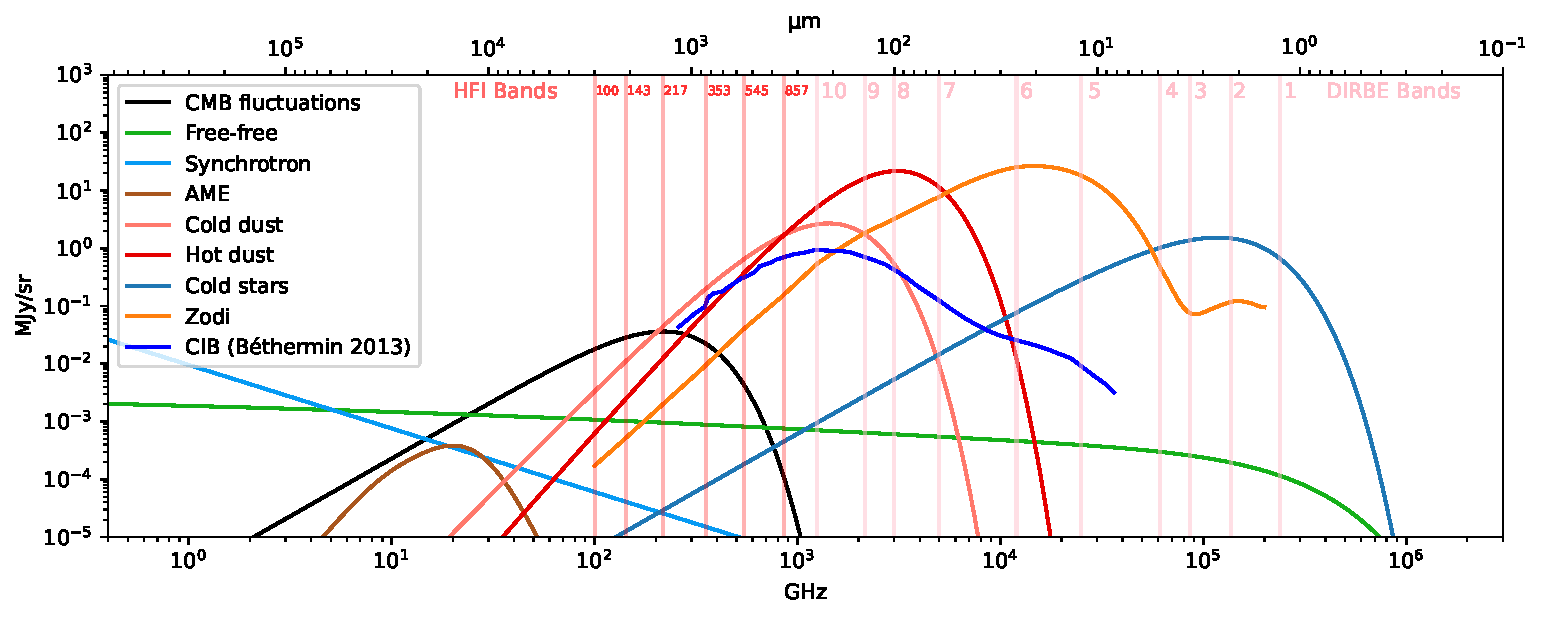
\includegraphics[width=\textwidth]{figs/sed/all_fgs.pdf}
  \caption{Components of the infrared temperature sky from 0.1$\mu$m to 1m wavelengths. The approximate contribution from stars is shown in blue, and the DIRBE and HFI band nominal frequencies are indicated by the vertical lines. The CIB estimate is taken from \cite{cibCurve}}
  \label{fig:sed}
\end{figure*}

In this paper, part of the larger Cosmoglobe DR2 results paper suite, we discuss the modelling of compact objects as part of our larger full sky astrophysical model. Section \ref{sec:models} discusses this modelling in a larger Bayesian context. Section \ref{sec:results} shows the astrophysical results of the work by presenting a unified star model and its associated errors. Section \ref{sec:consistency} then shows the consistency between our results and other work in this area. Finally, we conclude in Section \ref{sec:conclusions}, discussing the impacts of this work and offering some avenues for future research.

GAIA sed plot as a function of changing catalogue parameters

high level schematic diagram for intuition somehow of gaia, wise, beam and commander fit

histograms of stuff from gaia catalogue

\section{Compact Object modelling in a Bayesian context}
\label{sec:models}

In this work, we break the compact objects into three categories as follows: 1) Bright (> Mag 8 in the WISE 3.4 $\,\mu$m) objects with SEDs measured by Gaia (hereafter 'stars'), described in section \ref{sec:starmodel}, 2) Bright objects without SED information (hereafter 'extragalactic sources'), described in section \ref{sec:extragalacticmodel}, and 3) a diffuse background of dim objects (hereafter 'diffuse'), described in section \ref{sec:diffusemodel}.

Figure \ref{fig:starcount} shows the total number of stars and extragalactic objects in each pixel at nside=512. There are a total of 717454 stars supplemented with 3122 extragalactic sources over the full sky, but, as is expected, they are primarily clustered in the galactic plane. The majority of the sky contains 0-1 sources/pixel, making it well behaved. In the galactic plane, we have degeneracy between sources, which leads to instability in the individual star parameters, but the overall estimate of pointsource emission is quite stable, as shown in section \ref{sec:results}.

\begin{figure}
  \centering
  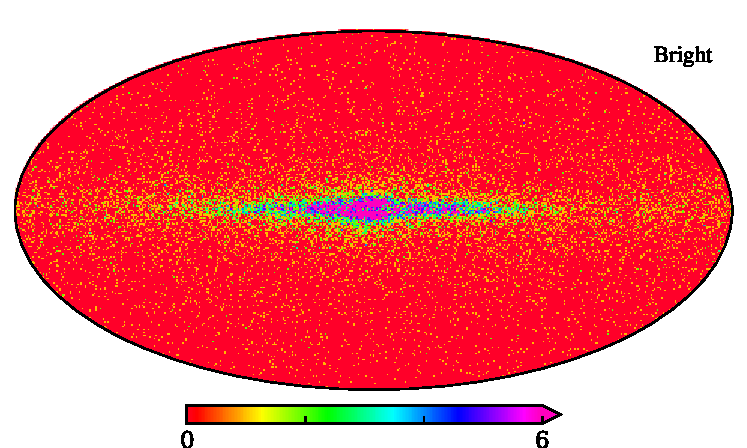
\includegraphics[width=\columnwidth]{figs/sourcecount/source_count.pdf}\\
  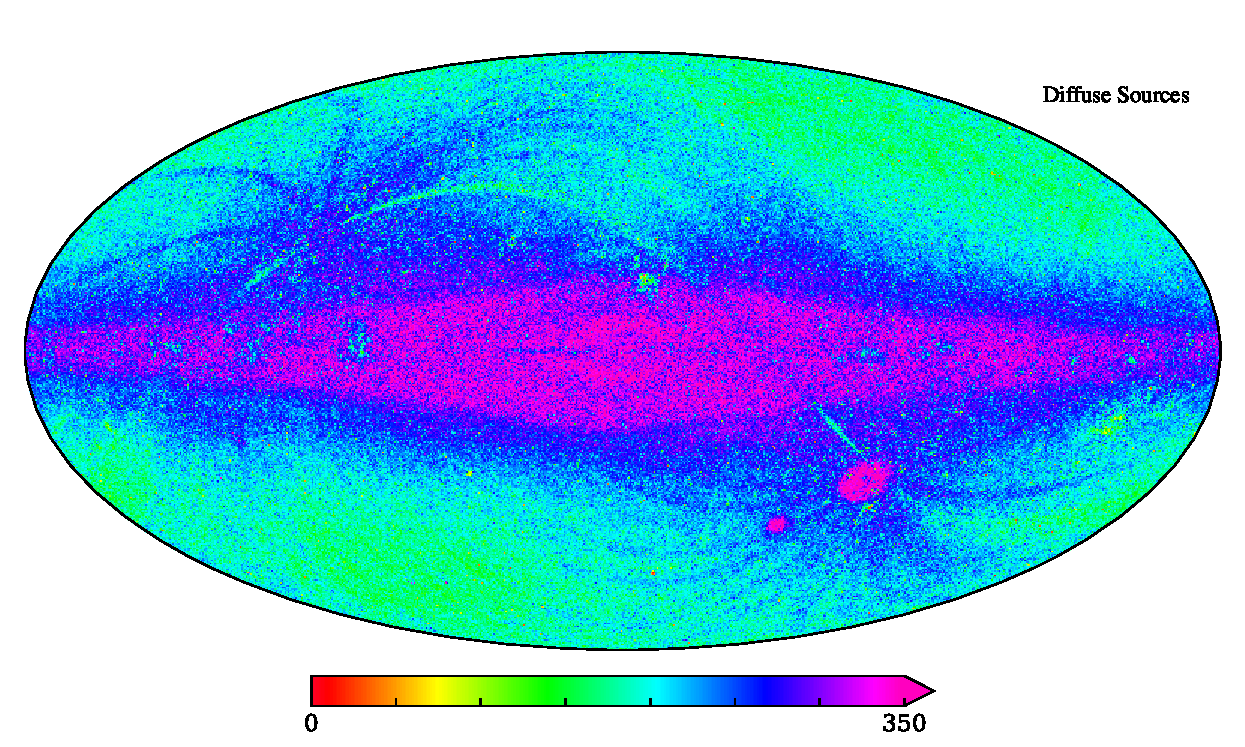
\includegraphics[width=\columnwidth]{figs/sourcecount/diffuse_count.pdf}
  \caption{The top panel shows the total number of bright sources in each pixel, counting both stars and extragalactic sources. The bottom panel is the total number of sources included in the diffuse template, which shows a clear imprint of the WISE scan strategy.}
  \label{fig:starcount}
\end{figure}

\subsection{Stars}

\label{sec:starmodel}

For each star we extract estimates of the effective temperature, $T_{\mathrm{eff}}$, the gravitational acceleration, $\log g$, and the metallicity, $[M/H]$, from the GAIA DR2 database \cite{gaiaCat}, and use those to identify a best-fit spectral energy density (SED) from the PHOENIX starlight database. 

The full Bayesian data mode is shown in \cite{CG02_01}, and includes the star component $s_{stars}(p, \lambda_j)$, the star emissions as a function of pixel $p$ and frequency $\lambda_j$ for a band $j$. Equation \ref{eq:datamodel} shows the data model for the star component that we describe in this paper


\begin{equation}
s_{stars}(p, \lambda_j) = \sum_i a_i B_i(p, \lambda_j) E_i(\lambda_j),
\label{eq:datamodel}
\end{equation}

where in the notation of \cite{CG02_01} 

\begin{equation}
f_{\mathrm{GAIA}} = B_i(p, \lambda_j) E_i(\lambda_j),
\end{equation}

which is the beam-convolved SED taken from the PHOENIX catalogue.

Here, we sum over each star $i$, where $a_i$ is a single overall amplitude parameter fit per star and $B_i(p, \lambda)$ is the instrument beam for a detector at frequency $\lambda$ in a pixel $p$ for a given star $i$. $E_i(\lambda)$ is the normalized emission for a given frequency $\lambda$. The emission $E_i$ is drawn directly from the GAIA data and the PHOENIX starlight database (see Sec. \ref{sec:catalogue}), and the beam $B$ is fixed for each detector, so we fit only the overall amplitude $a_i$ for each star in this model. This greatly reduces the degeneracies between the stars and other astrophysical components such as dust, and was found to work better than fitting a full SED per star. We include a star component in DIRBE bands 01-06, as at longer wavelengths the contribution from star emission was greatly subdominant to zodiacal light and dust, and including that data degraded the quality of the amplitude fits. 

To sample the star amplitudes $a_i$ we attempt to minimize the residual in each band for each source $i$

\begin{equation}
\label{eq:minimize}
X_ia_i - Y_i = 0.
\end{equation}

The solution is just the mapmaking equation, where

\begin{equation}
X_i = S^T N^{-1} S = \sum_{j,p}\frac{E_{ij}^2 B^2_{ij}(p)}{\sigma_j^2(p)} 
\end{equation}

and

\begin{equation}
Y_i = S^TN^{-1}d = \sum_{j,p} \frac{E_{ij}B_{ij}(p) d_j(p)}{\sigma_j^2(p)}.
\end{equation}

Here, $\sigma_j^2(p)$ is the noise in pixel $p$ in band $j$, and $d_j(p)$ is the data map in band $j$ at pixel $p$. To reduce degeneracies, we fit the point sources on a data map with all other astrophysical components already removed, so $d_j(p)$ contains only noise and the point source $i$. The solution to \ref{eq:minimize} is simply $a_i = \frac{Y_i}{X_i}$, which gives a single overall amplitude for each star $i$. To sample the amplitudes, we also include a fluctuation term, such that our final sample for the amplitudes is given by

\begin{equation}
a_i = \frac{Y_i}{X_i} + \frac{1}{\sqrt{X_i}} N_i(0,1),
\end{equation}

where $N_i(0,1)$ is a sample drawn from a unit Gaussian with 0 mean.

\subsection{Extragalactic Pointsources}

\label{sec:extragalacticmodel}

After fitting the star catalogue, we are left with another background of pointsources, those with extragalactic origins. Sources that do not match against the GAIA catalogue or that do not have sufficient SED information to model, but which are still brighter than magnitude 5.06 in the WISE $3.4 \mu m$ band ($3000$ MJy in DIRBE 01) are fit with a more general blackbody of the form:

\begin{equation}
\frac{e^{\frac{\nu_0 h}{k_b \theta}} - 1}{e^{\frac{\nu h}{k_b \theta}} - 1} * (\frac{\nu}{\nu_0})^{\theta_2 + 1}
\end{equation}

Here, $\nu_0$ is a reference frequency, set to $239833.966$ GHz (1.25 $\mu m$). 



\subsection{Diffuse Star Emission}

\label{sec:diffusemodel}

Finally, after modelling the brightest sources using one of the two methods described above, we are left with a diffuse background of stars that are too dim to be individually resolved, but that can still couple to other parameters such as the band monopoles and so must be accounted for. We model this diffuse background using a single full-sky template, generated from the WISE W1 data. We take the full AllWISE pointsource catalog, and for each source with a included W1 magnitude that isn't already included in one of the previous pointsource models (ie. sources dimmer than Mag. 5) we create a high resolution healpix map \citep{healpix} at nside=2048. Adding each source in turn to this map, we then downgrade to nside=512, which gives the map shown in Fig. \ref{fig:diffuse}. 

\begin{figure}
  \centering
  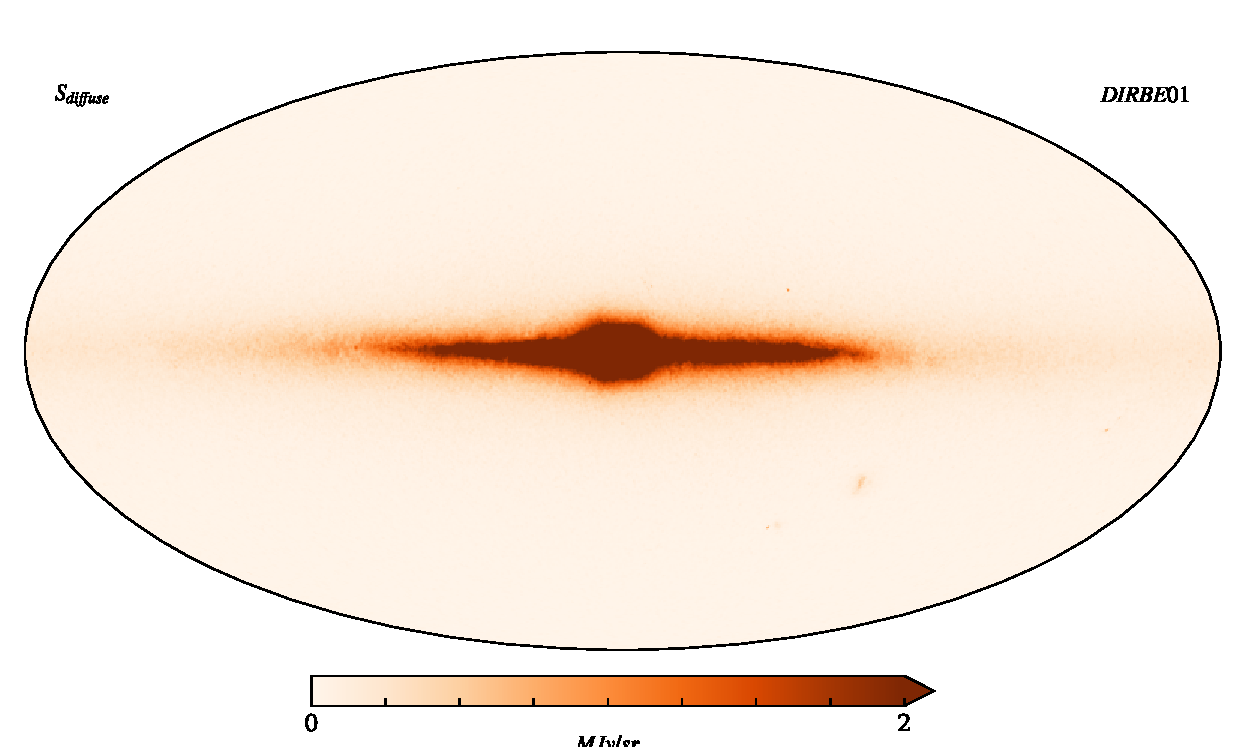
\includegraphics[width=\columnwidth]{figs/diffuseTemplate/diffuse_stars.pdf}\\
  \caption{The template of diffuse star emission evaluated in the DIRBE 01 band.}
  \label{fig:diffuse}
\end{figure}

This template is then included in the full sky model, and fit jointly in bands 01-04, with an SED given by the mean of all SEDs of stars modelled in section \ref{sec:starmodel}. This SED is fit with a single amplitude parameter, which compensates for the overall difference in bandpass between W1 and the DIRBE bands. The mean of this SED averaged over all the samples in the full chain is shown as the red line in Fig. \ref{fig:starSEDs}.

\subsection{Priors}

\section{Astrophysical results}
\label{sec:results}

\subsection{Maps}

In Figure \ref{fig:starsT} we show the mean compact object maps for the full pipeline run in all six DIRBE bands where they are modelled. Here, the maps show the sum of star component, the extragalactic source component, and the diffuse background, which fully accounts for the pointsource emission over the full sky.

\begin{figure*}
  \centering
  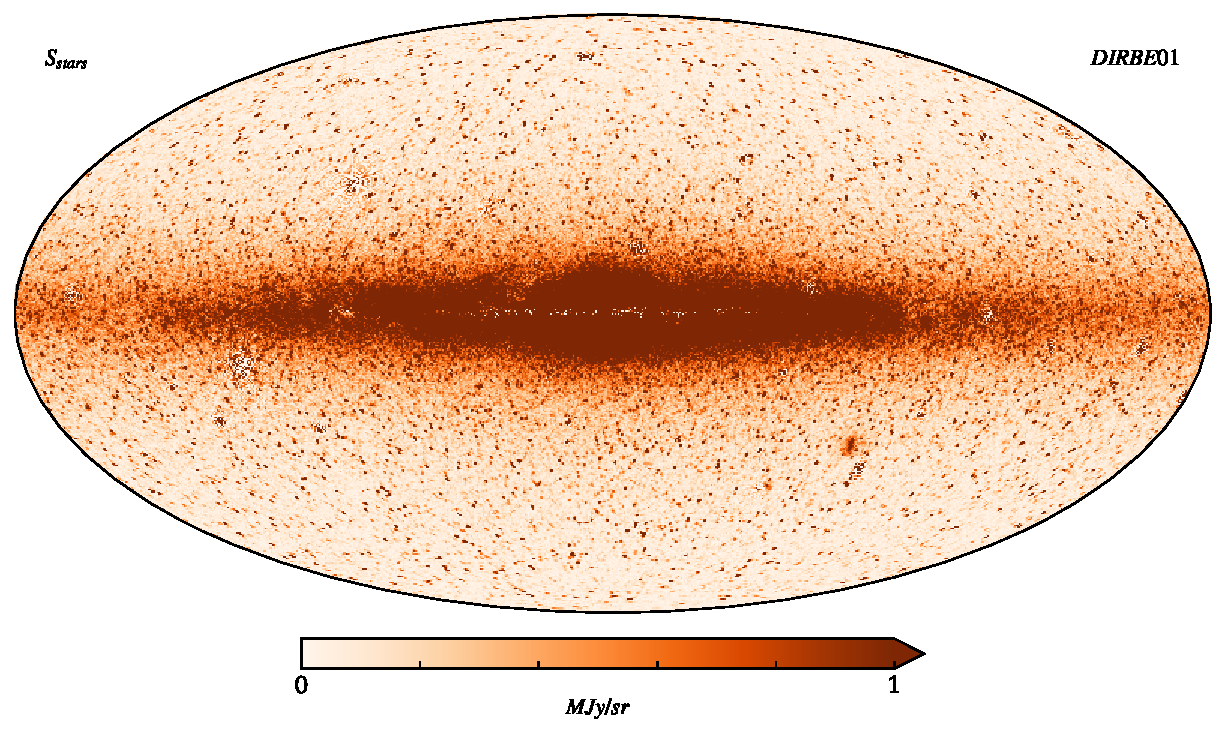
\includegraphics[width=0.49\textwidth]{figs/starmaps/all_stars_mean_01.pdf}
  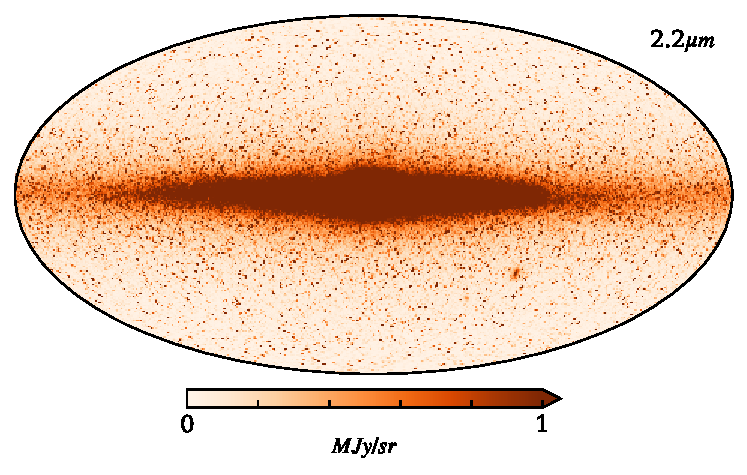
\includegraphics[width=0.49\textwidth]{figs/starmaps/all_stars_mean_02.pdf} \\
  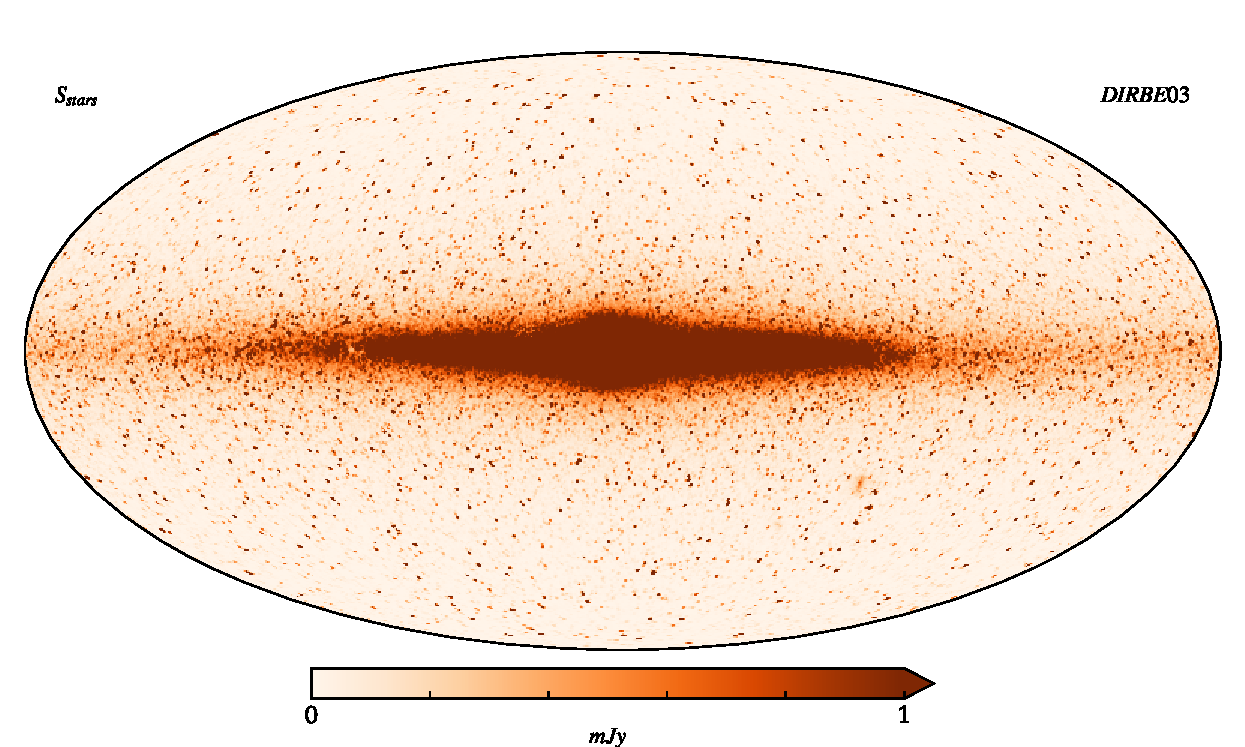
\includegraphics[width=0.49\textwidth]{figs/starmaps/all_stars_mean_03.pdf}
  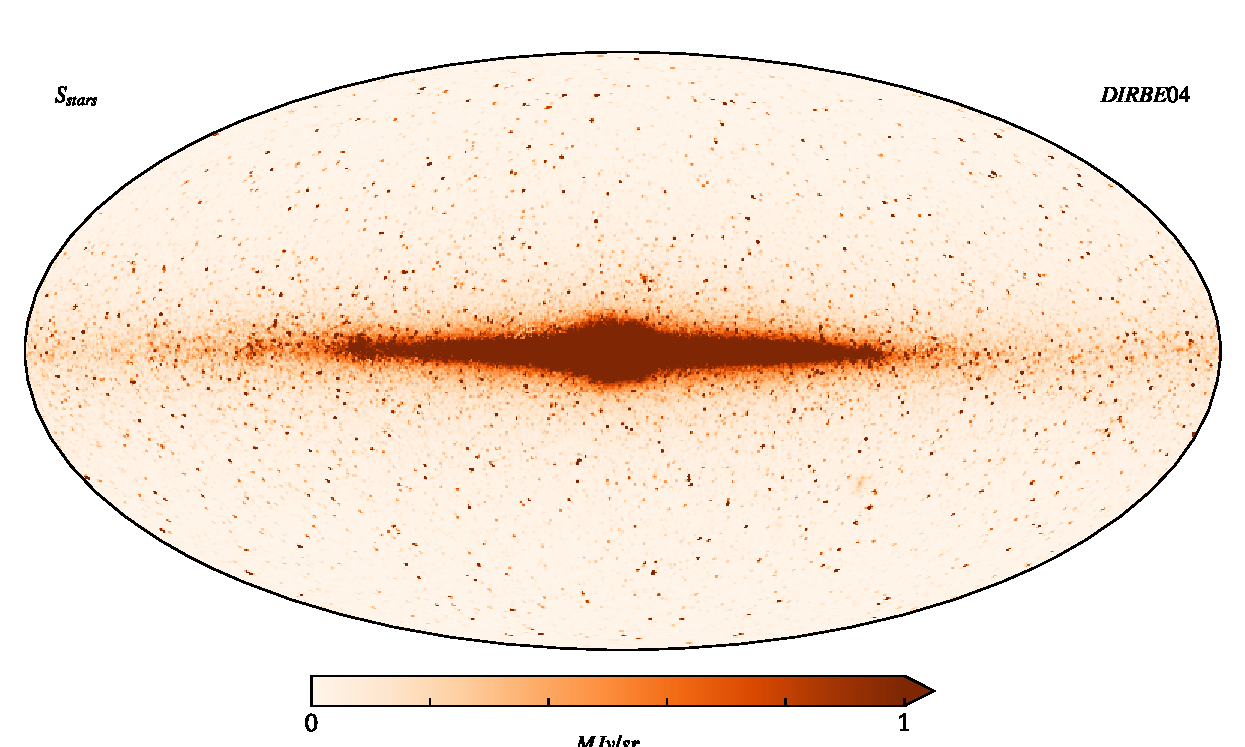
\includegraphics[width=0.49\textwidth]{figs/starmaps/all_stars_mean_04.pdf} \\
  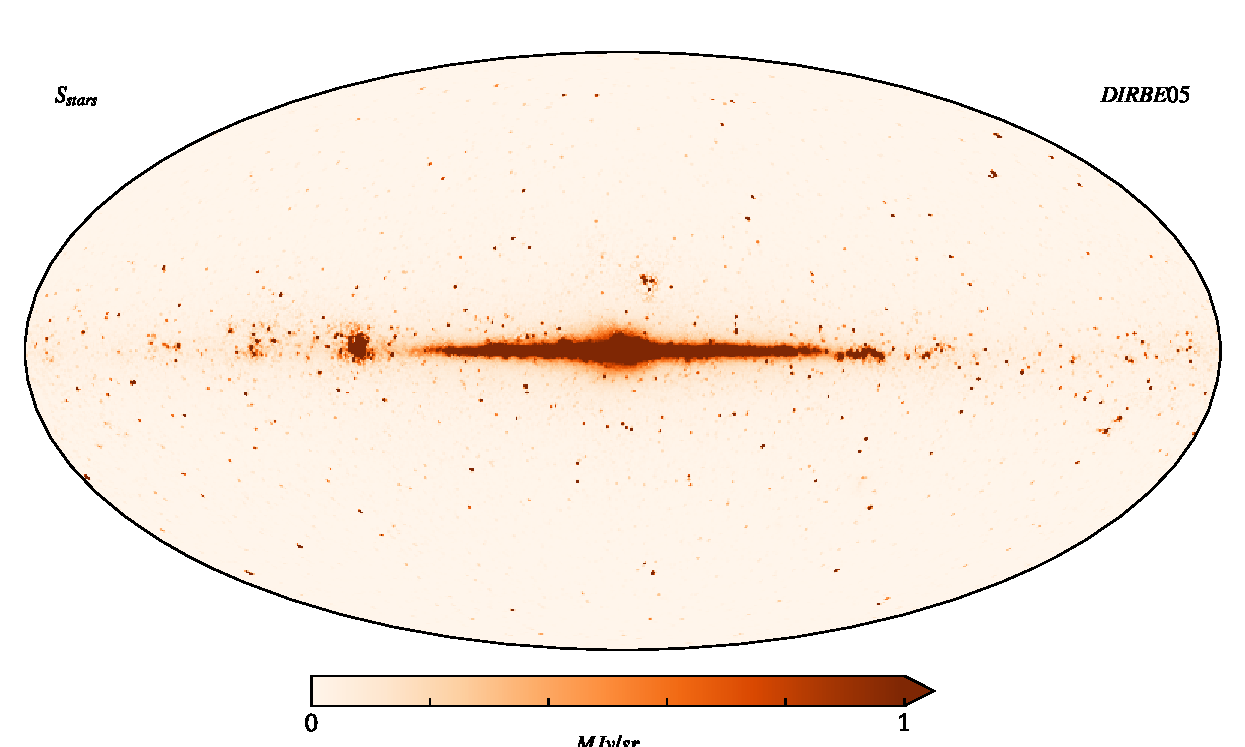
\includegraphics[width=0.49\textwidth]{figs/starmaps/all_stars_mean_05.pdf}
  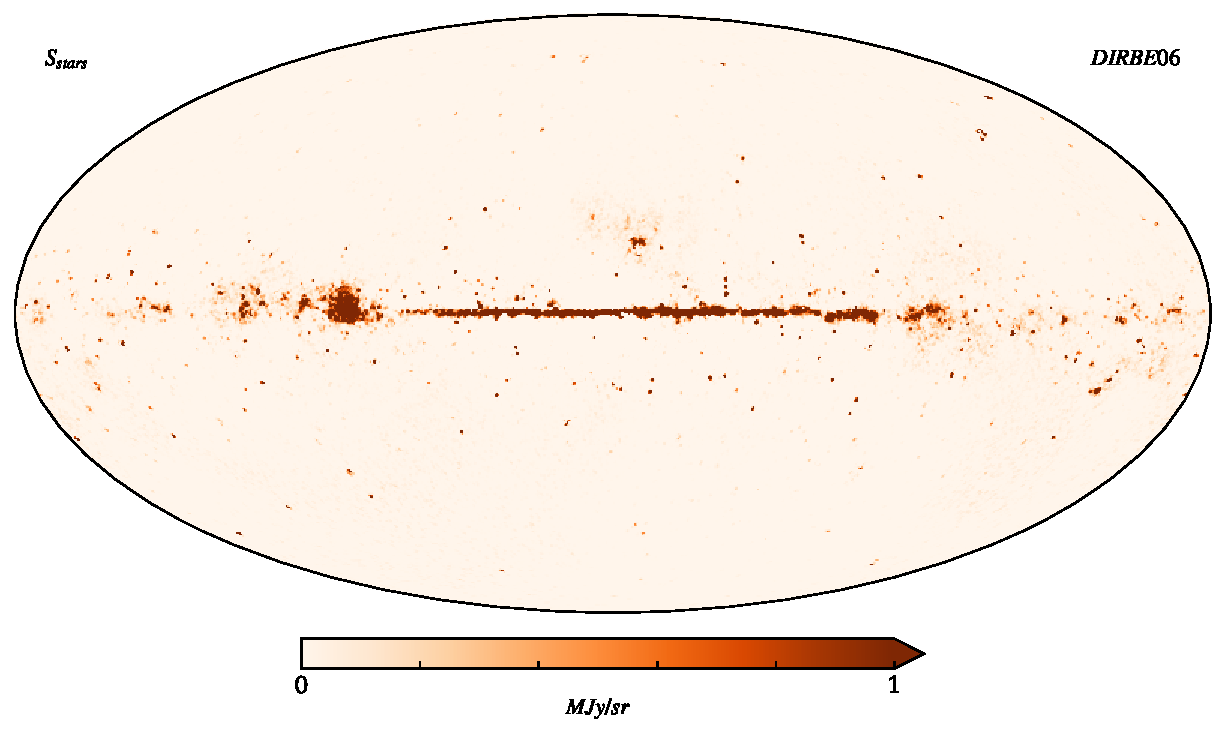
\includegraphics[width=0.49\textwidth]{figs/starmaps/all_stars_mean_06.pdf} \\
  \caption{Mean compact object maps from the Cosmoglobe DR2 release for the first 6 DIRBE bands. }
  \label{fig:starsT}
\end{figure*}

In Figure \ref{fig:zooms} we show zoom ins of a 20$^o$ patch of sky centered at (lon, lat)= $20^o, 50^o$, plotting the sky map in each band, the star model and the resulting residual after removing the sky model from the data.

\begin{figure*}
  \centering
  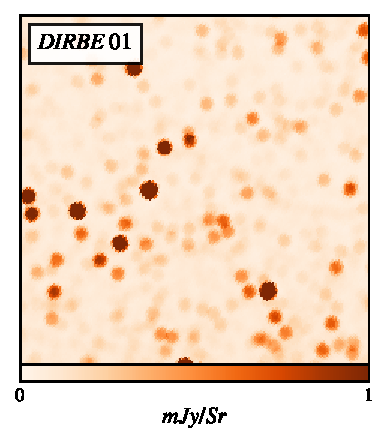
\includegraphics[width=0.31\textwidth]{figs/zoom/bandmap_01.pdf}
  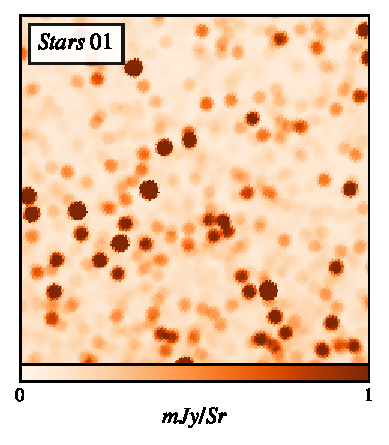
\includegraphics[width=0.31\textwidth]{figs/zoom/starmap_01.pdf}
  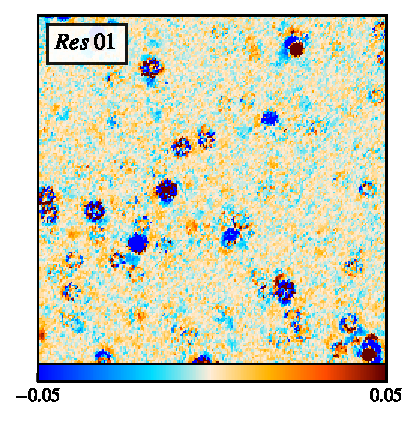
\includegraphics[width=0.33\textwidth]{figs/zoom/resmap_01.pdf}\\
    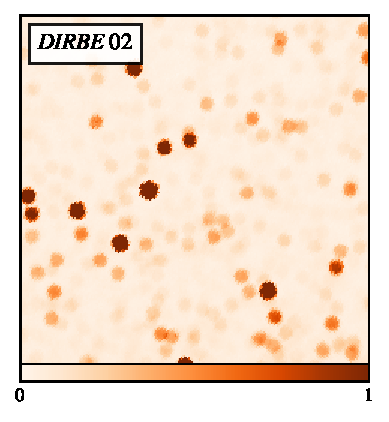
\includegraphics[width=0.31\textwidth]{figs/zoom/bandmap_02.pdf}
  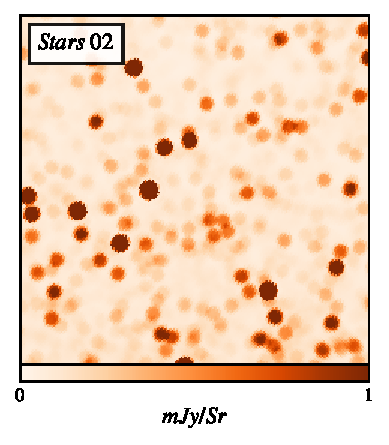
\includegraphics[width=0.31\textwidth]{figs/zoom/starmap_02.pdf}
  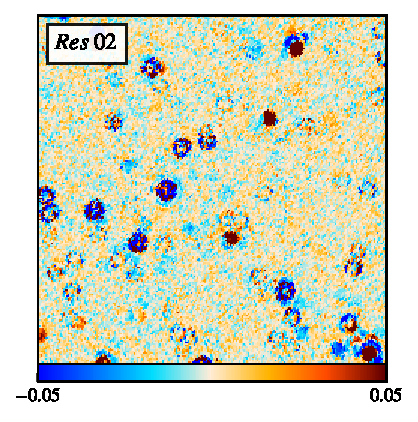
\includegraphics[width=0.33\textwidth]{figs/zoom/resmap_02.pdf}\\
    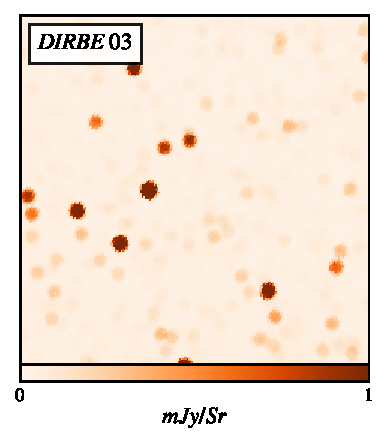
\includegraphics[width=0.31\textwidth]{figs/zoom/bandmap_03.pdf}
  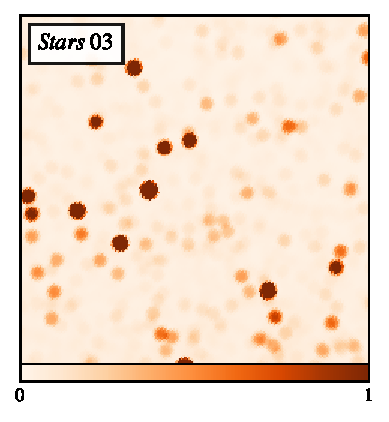
\includegraphics[width=0.31\textwidth]{figs/zoom/starmap_03.pdf}
  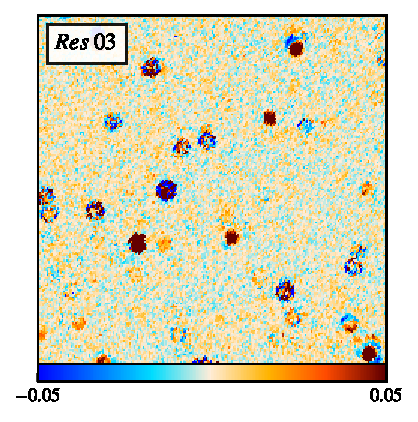
\includegraphics[width=0.33\textwidth]{figs/zoom/resmap_03.pdf}\\
    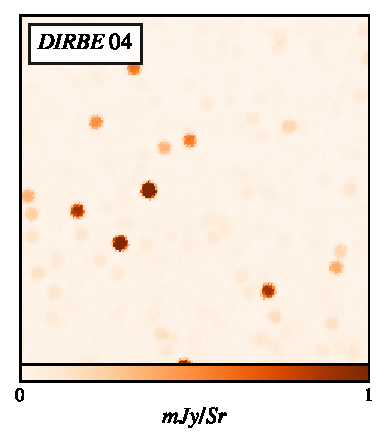
\includegraphics[width=0.31\textwidth]{figs/zoom/bandmap_04.pdf}
  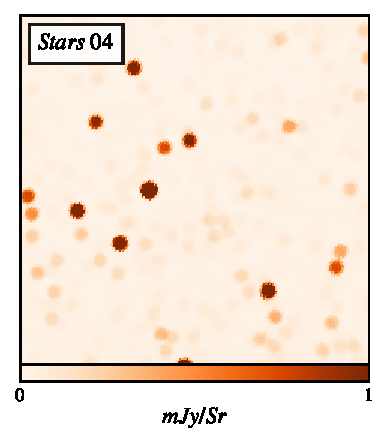
\includegraphics[width=0.31\textwidth]{figs/zoom/starmap_04.pdf}
  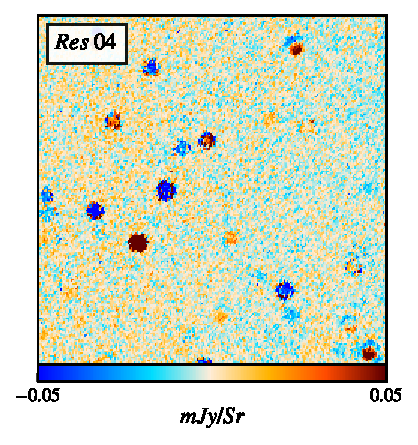
\includegraphics[width=0.33\textwidth]{figs/zoom/resmap_04.pdf}\\

  \caption{Zoom-ins on a subregion of the sky centred at (20,50) }
  \label{fig:zooms}
\end{figure*}


In Figure \ref{fig:amptrace}, we show the summed amplitude of the compact sources in three pixels in different regions in the sky. The first 25 samples in each chain are discarded as burn in, and the remaining samples (233 in total) form the samples in our analysis. We see good mixing of the total amplitudes, although due to degeneracies in the model especially in the galactic plane, plotting individual parameters show that they are trading off between each other in unpredictable ways, which is why we show only the total signal, which is stable.

\begin{figure*}
  \centering
  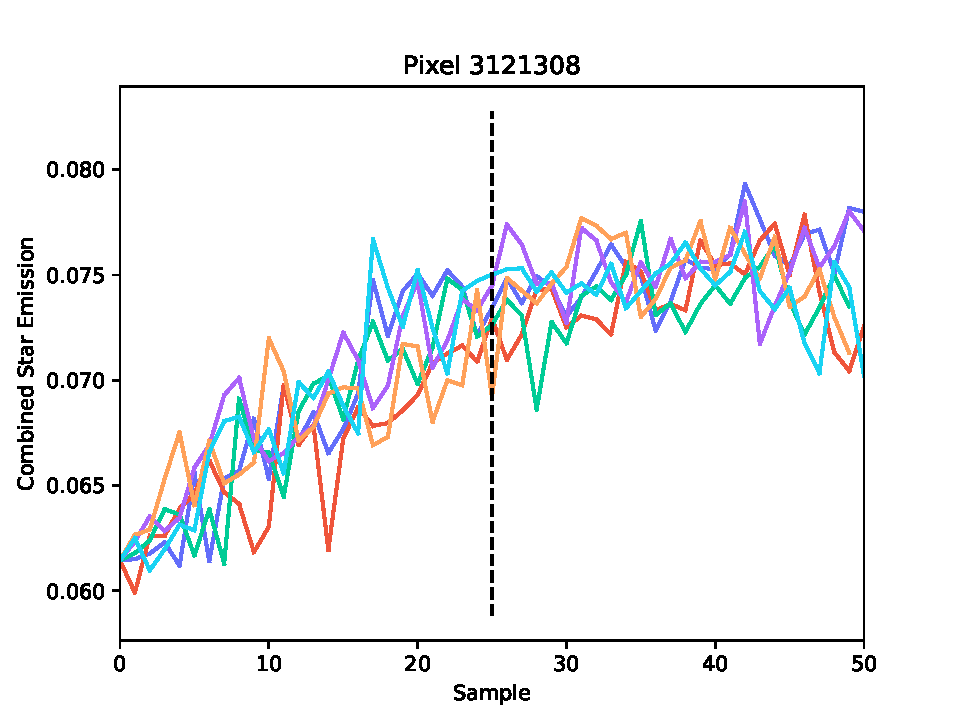
\includegraphics[width=0.33\textwidth]{figs/mixing/total_star_trace_3121308.pdf} 
  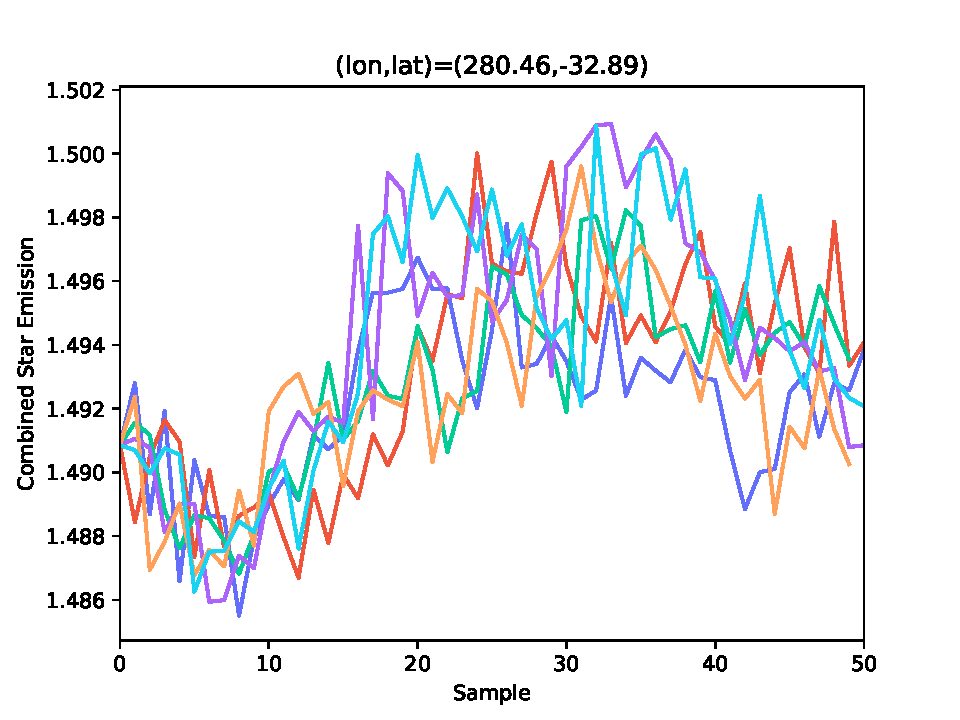
\includegraphics[width=0.33\textwidth]{figs/mixing/total_star_trace_2429499.pdf}
  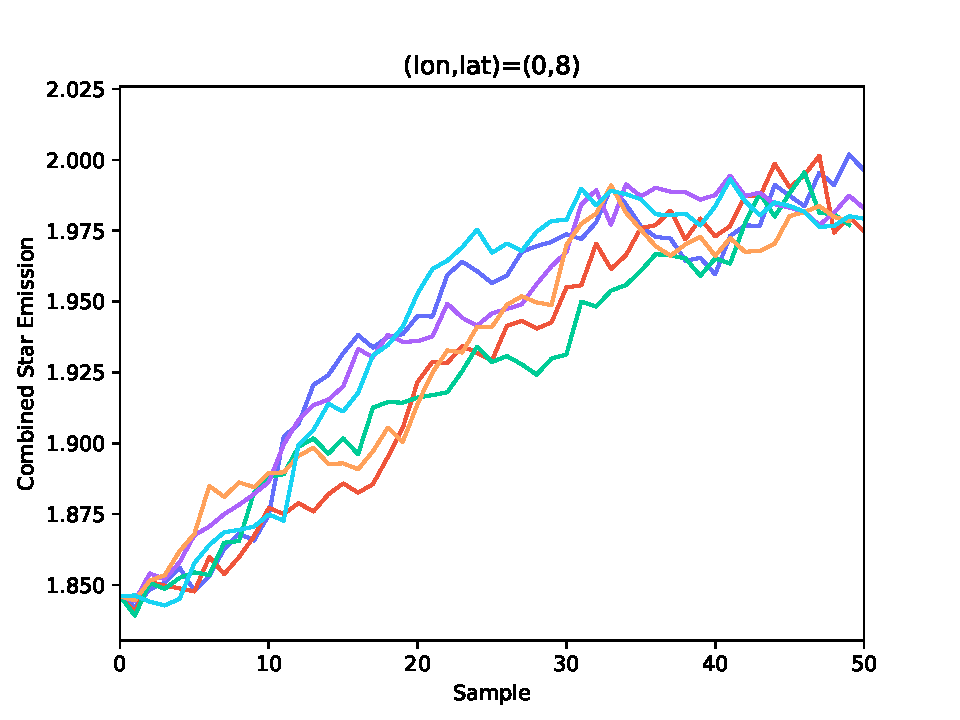
\includegraphics[width=0.33\textwidth]{figs/mixing/total_star_trace_1352704.pdf}\\
   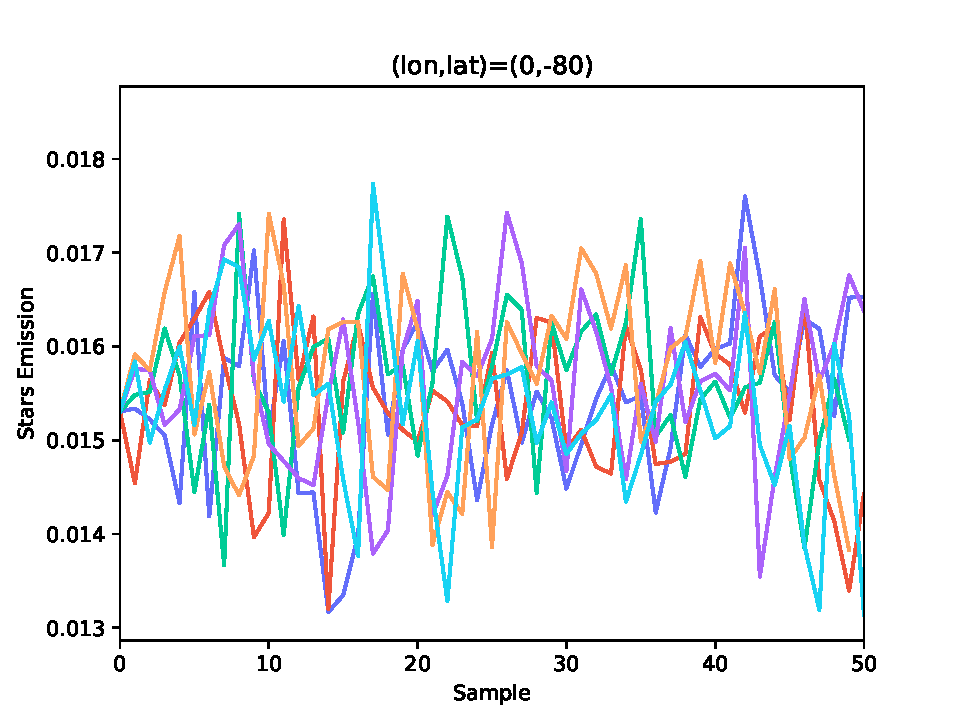
\includegraphics[width=0.33\textwidth]{figs/mixing/star_trace_3121308.pdf} 
  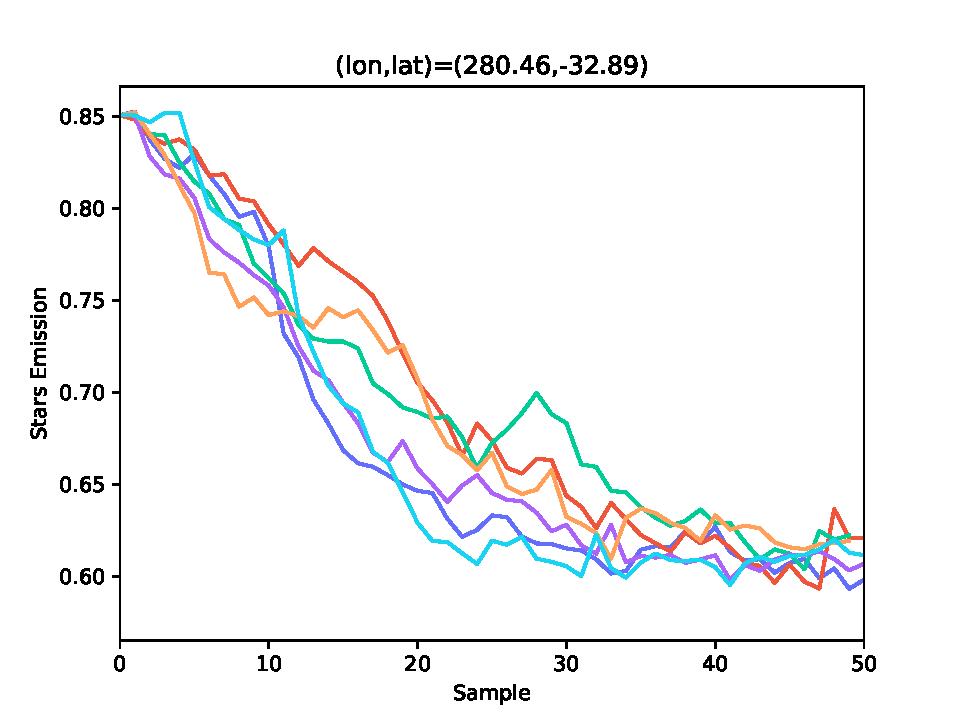
\includegraphics[width=0.33\textwidth]{figs/mixing/star_trace_2429499.pdf}
  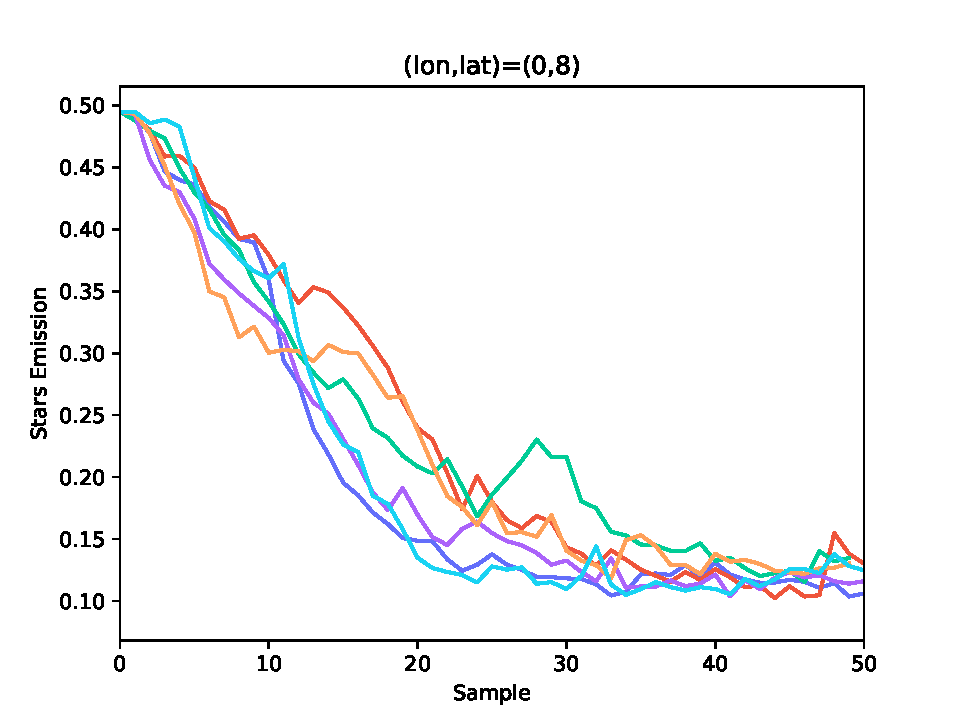
\includegraphics[width=0.33\textwidth]{figs/mixing/star_trace_1352704.pdf}\\
    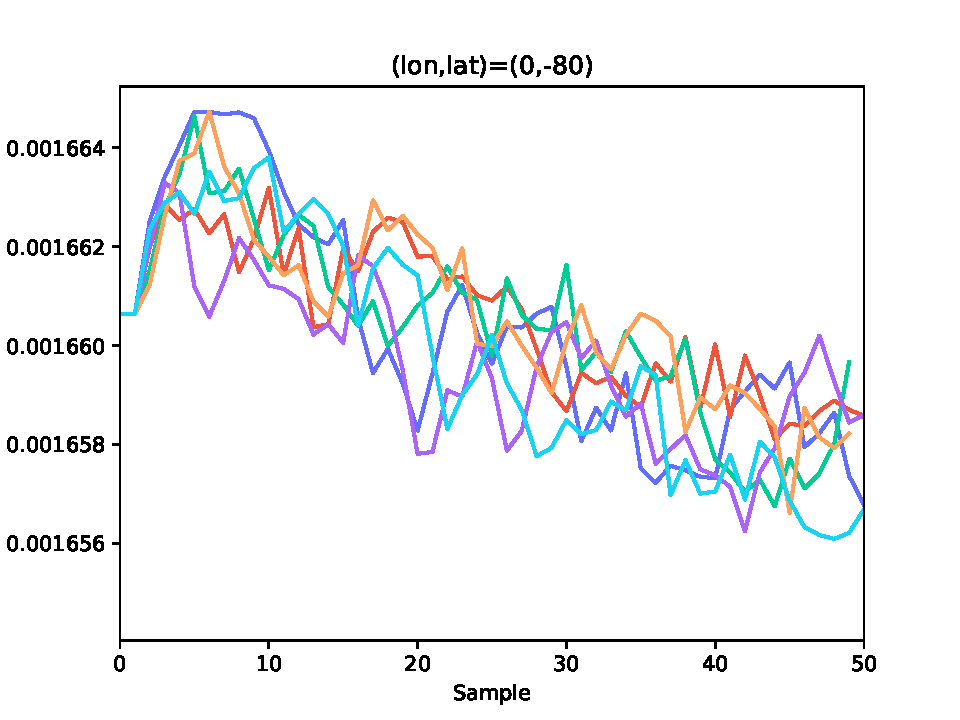
\includegraphics[width=0.33\textwidth]{figs/mixing/exgal_trace_3121308.pdf} 
  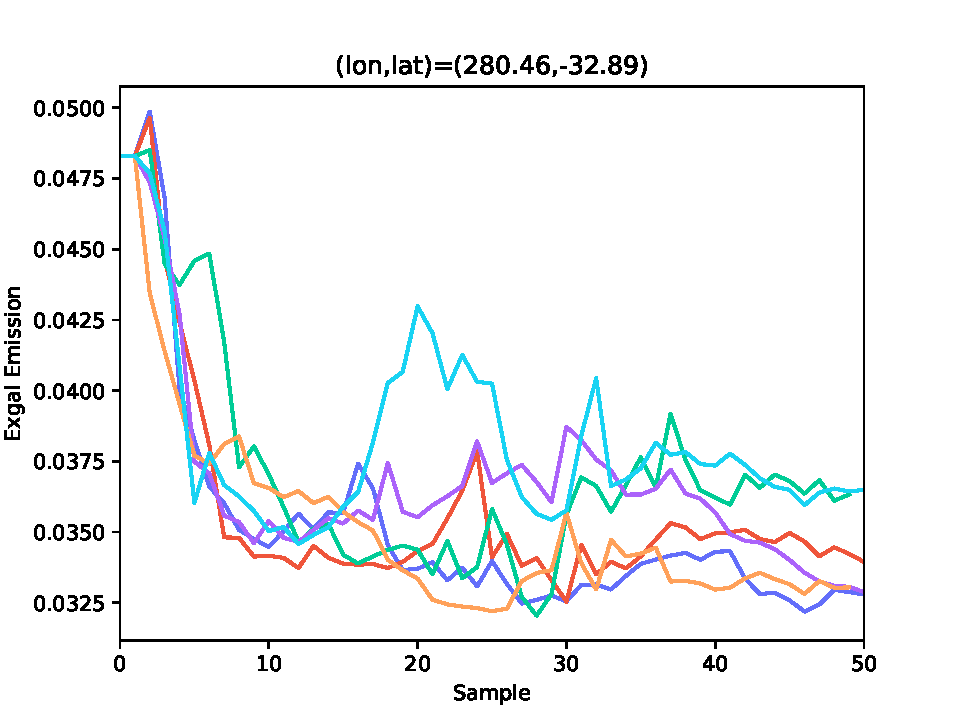
\includegraphics[width=0.33\textwidth]{figs/mixing/exgal_trace_2429499.pdf}
  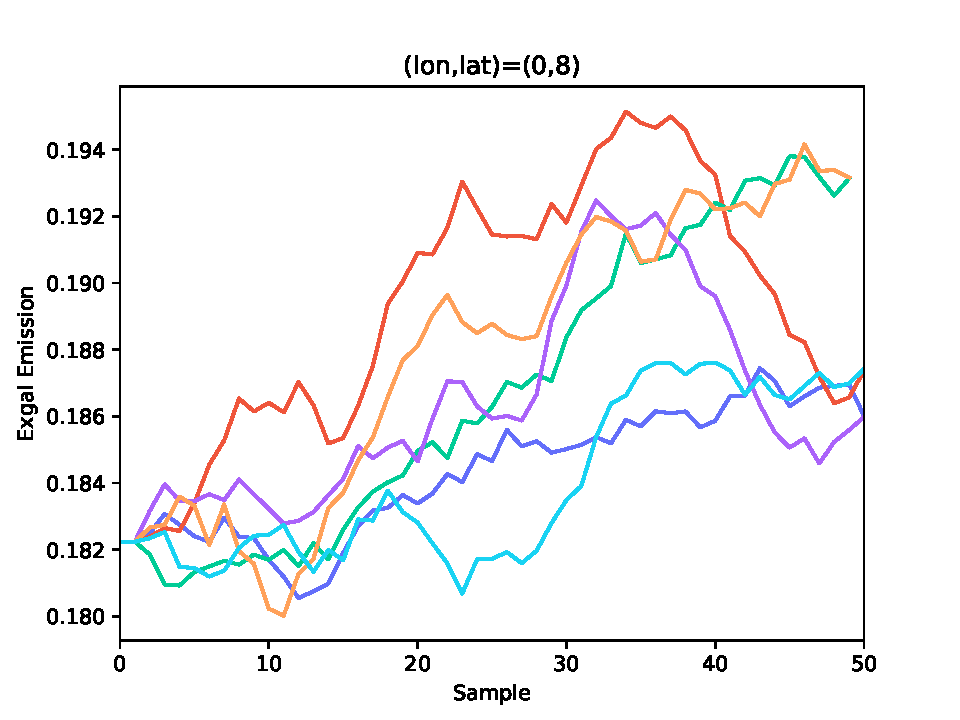
\includegraphics[width=0.33\textwidth]{figs/mixing/exgal_trace_1352704.pdf}\\
    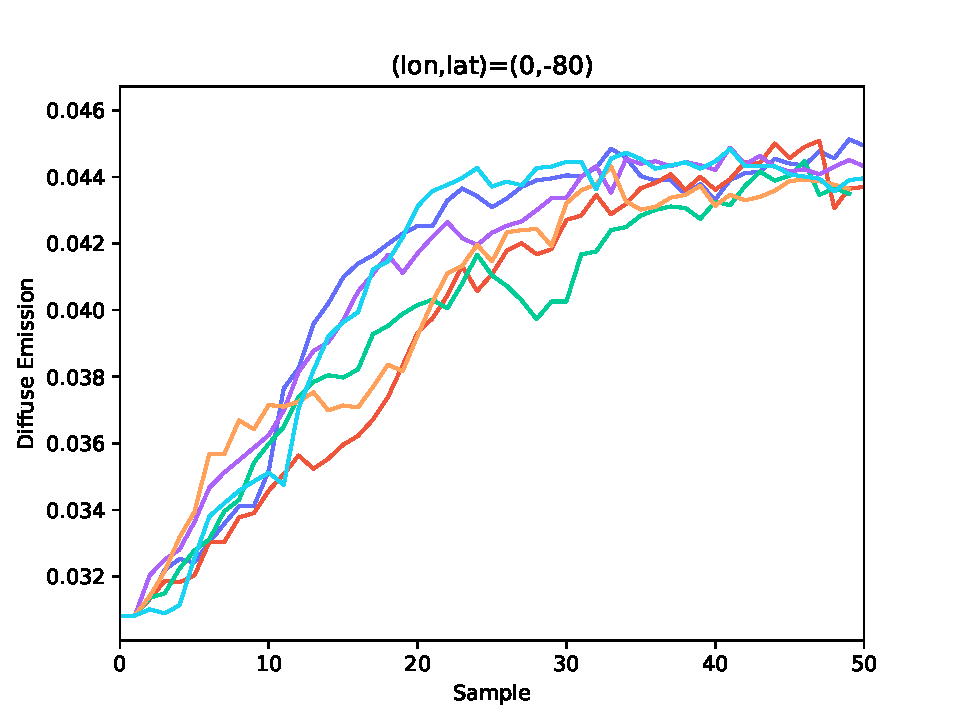
\includegraphics[width=0.33\textwidth]{figs/mixing/diffuse_trace_3121308.pdf} 
  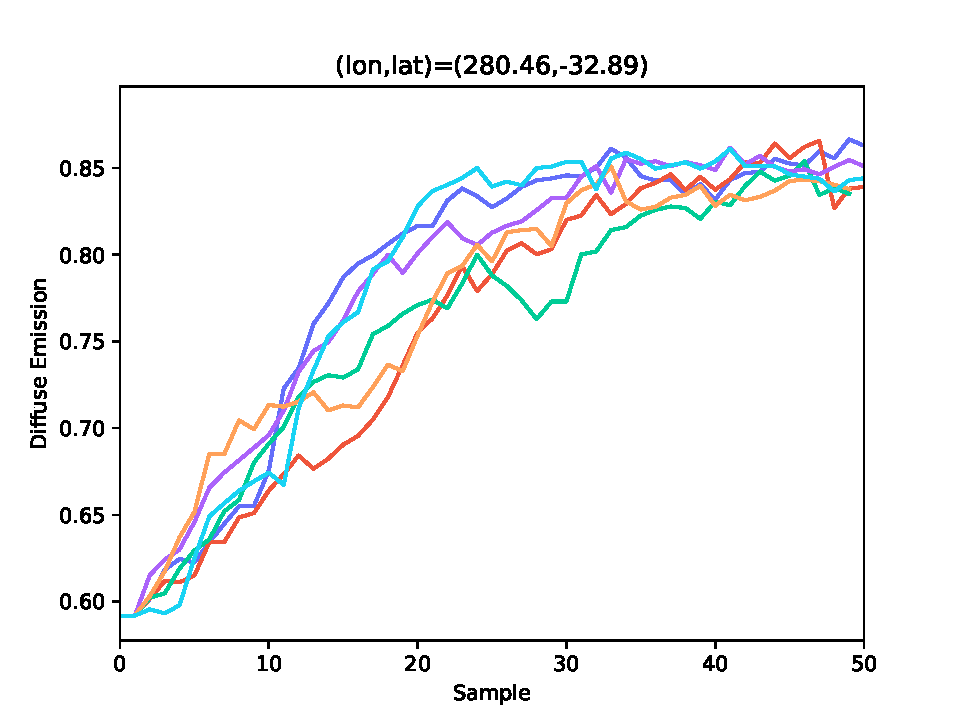
\includegraphics[width=0.33\textwidth]{figs/mixing/diffuse_trace_2429499.pdf}
  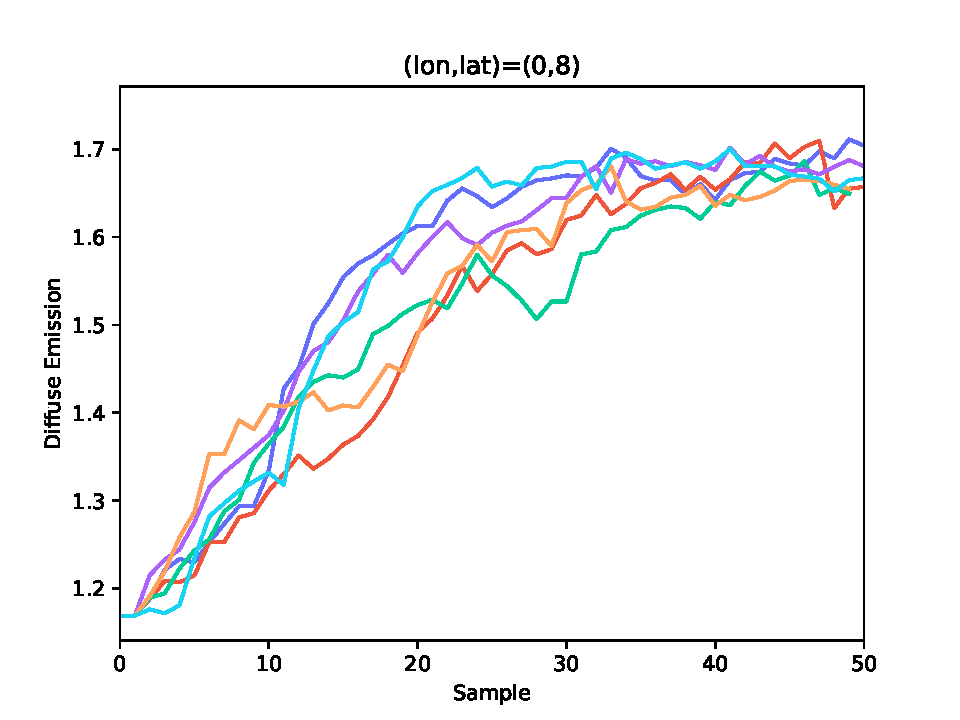
\includegraphics[width=0.33\textwidth]{figs/mixing/diffuse_trace_1352704.pdf}\\
  \caption{Trace plots of the total star amplitude for three pixels in different regions of the sky in DIRBE band 01. The dashed vertical line indicates the end of the burn in period, and samples after that are included in our final sample set.}
  \label{fig:amptrace}
\end{figure*}

correlation plot

\subsection{Spectral Energy Densities}

Figure \ref{fig:starSEDs} shows the SED models for all 717454 star sources in our catalogue, as well as the full sky mean SED, which is used as the SED for the diffuse component. 

\begin{figure}
  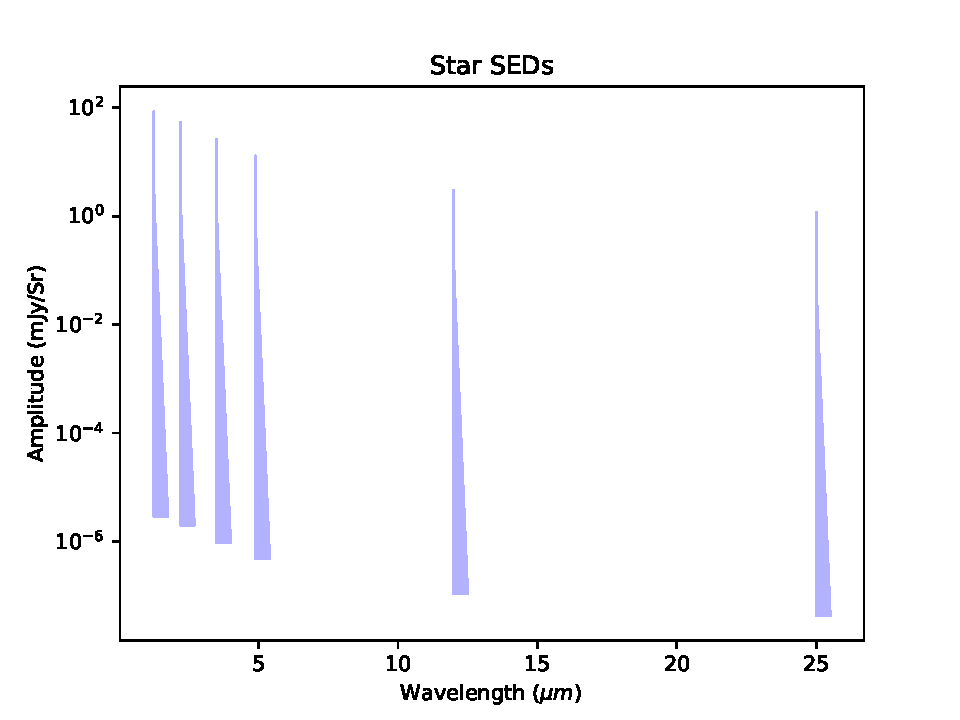
\includegraphics[width=\columnwidth]{figs/starseds/star_seds.pdf}
  \caption{Star emission as a function of wavelength. In blue we have the distributions of amplitudes for each source in our catalogue as a function of frequency. Each star has a fixed SED that is fit with a single amplitude parameter, and after this fitting process we obtain the distributions shown here at each frequency. Overplotted in red is the full sky mean of all SEDs, which is used as the SED for the diffuse template. The fitting process prefers a much higher amplitude for this diffuse component, which leads to the diffuse SED being greater than the mean of each individual star.}
  \label{fig:starSEDs}
\end{figure}

SEDs for extragalactic sources


\section{Comparison to other Analyses}
\label{sec:consistency}

The original DIRBE analysis team \citep{dirbeFaint} also removed point sources from their measurement of the CIB emission, but followed a different approach. Instead of modelling the bright sources, the original analysis simply masked pixels brighter than a threshold (15 Jy in band 01), which resulted in cutting almost 35 \% of the sky at 1.25 $\mu$m. For the diffuse sources, they build a model (the 'faint source model' or FSM) using the mechanism of \cite{wainscoat}, which integrates a model of source counts over the full, including models of galactic morphology, 87 discrete source types and the contribution from dust extinction. The results of this model in the DIRBE 01 band are shown in Figure \ref{fig:DIRBEfaint}, as well at the difference between our faint source model and theirs, evaluated in that same band. 

\begin{figure}
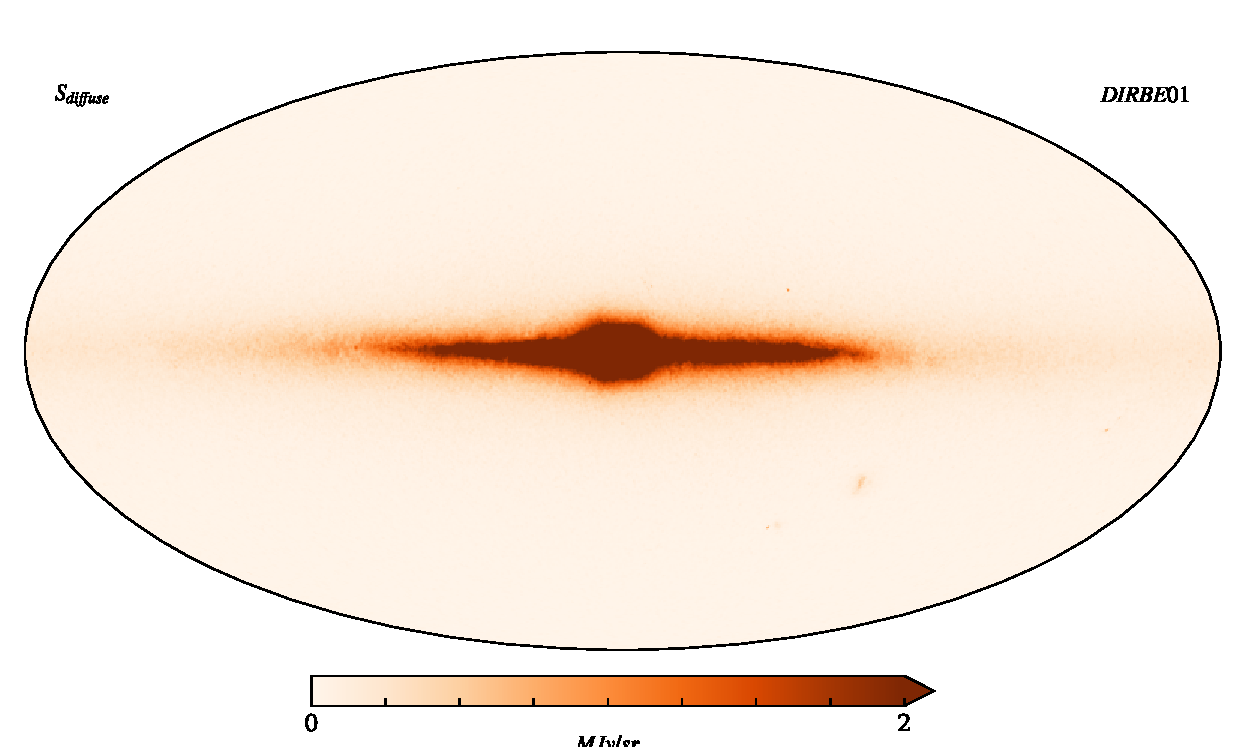
\includegraphics[width=\columnwidth]{figs/diffuseTemplate/diffuse_stars.pdf}
  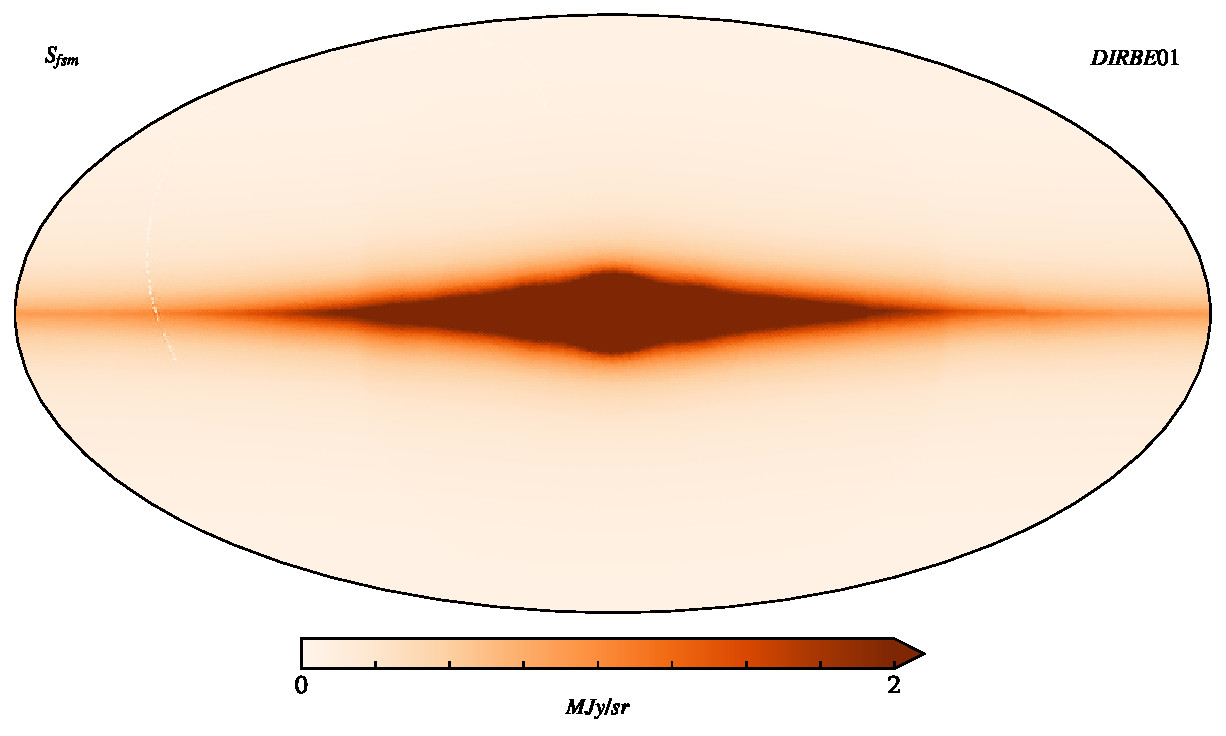
\includegraphics[width=\columnwidth]{figs/diffuseTemplate/dirbe_template.pdf}\\
  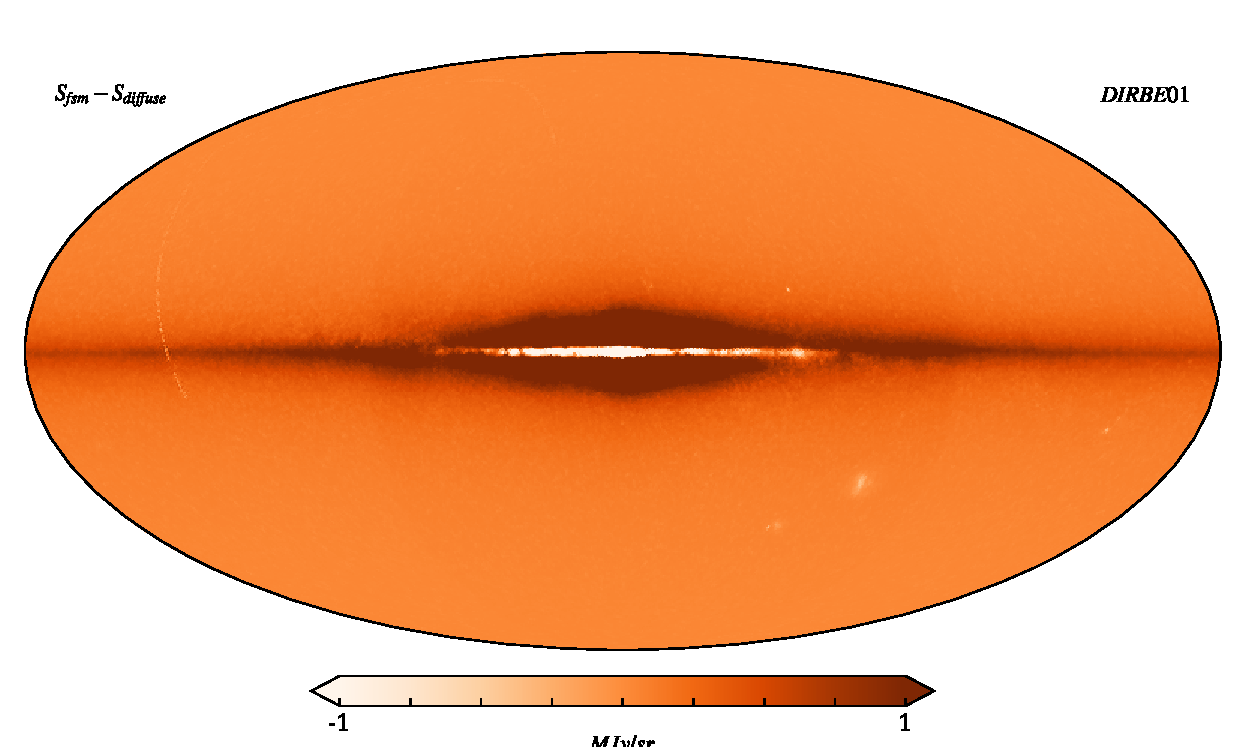
\includegraphics[width=\columnwidth]{figs/diffuseTemplate/diffuse_diff.pdf}\\
  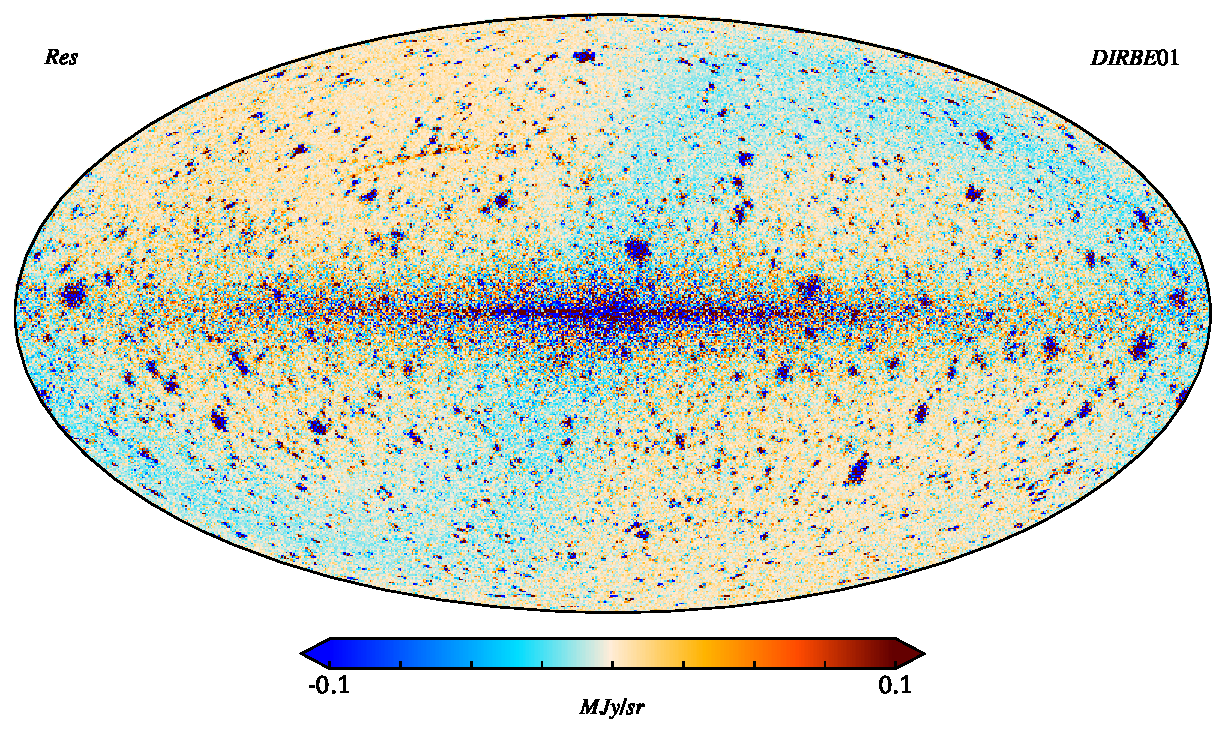
\includegraphics[width=\columnwidth]{figs/diffuseTemplate/band01_res.pdf}\\
  \caption{The Commander diffuse star template reproduced from fig. \ref{fig:diffuse} (Top). The DIRBE faint star model at 1.25 $\mu$m retrieved from LAMBDA and converted from QuadCube to healpix (position 2) and the difference between that model and the Cosmoglobe star model used in this analysis (position 3). The bottom panel shows the DIRBE 01 residual from the Commander run, which shows that our star model is slightly overestimating signal in the galactic plane.}
  \label{fig:DIRBEfaint}
\end{figure}

This difference shows that the DIRBE FSM predicts more star emission in the galactic plane than the integrated AllWISE pointsource catalogue, except in the very inner part of the plane where dust extinction is dominant. The AllWISE data was found to be complete to Mag 17, so it is possible that a large number of fainter sources are missing, which could cause an underestimate of the total star emission. Dust extinction is also not explicitly included in our star model, although should be implicitly accounted for due to the missing and dimmer catalogue sources within that region. The bottom panel of fig. \ref{fig:DIRBEfaint} shows the Commander DIRBE 01 residuals, averaged over the full chain. The blue area in the galactic plane shows that when fit against the data, our current star model overestimates the galactic emission in this band, indicating that the DIRBE FSM with its even higher estimate would be a worse fit to the data. 

After the official DIRBE analysis, \cite{DIRBE2mass}, following \cite{gorjian} used the 2MASS catalogue to remove star emissions from DIRBE and find an improved upper limit on the CIB monopole, but were ultimately unable to claim a detection due to the zodiacal light contamination that they were unable to fully correct. Their analysis looked at four dark patches of the sky and used 2MASS to estimate the contribution of both bright (K band magnitude > 14) and faint sources to the total signal in each patch, which we can compare with the Cosmoglobe estimates, as shown in Table \ref{tab:2mass}.

\begin{table*}
    \centering
    \newcolumntype{C}{ @{}>{${}}r<{{}$}@{} }
    \begin{tabular}{l c c c c c c c c c}
    \hline
    \hline
     Patch & $l$ & $b$ & $r$ & \multicolumn{2}{c}{Bright Stars} & \multicolumn{2}{c}{Diffuse Stars} & \multicolumn{2}{c}{Galaxies} \\ 
     & ($^{\circ}$) & ($^{\circ}$) & ($^{\circ}$) & \multicolumn{2}{c}{(kJy/sr)} & \multicolumn{2}{c}{(kJy/sr)} & \multicolumn{2}{c}{(kJy/sr)} \\
          &  & & & \cite{DIRBE2mass} & CG & \cite{DIRBE2mass} & CG & \cite{DIRBE2mass} & CG\\
    
     \hline
     1 \rule{0pt}{2ex} & 127.3 & 63.8  & 1.5 & 48.23 & 23.7 & 3.08 & 64.6 & 0.1 & 2.1\\
     2 & 107.7 & 57.7 & 2.0 & 58.86 & 29.2 & 3.62 & 80.6 & 0.1 & 2.1 \\
     3 & 157.0 & -26.0 & 2.0 & 51.48 & 93.7 & 2.94 & 167.7 & 0.1 & 59.2 \\
     4 & 257.8 & -59.4 & 1.9 & 70.01 & 38.5 & 3.92 & 83.9 & 0.1 & 9.5\\
     \hline
    \end{tabular}
    \caption{Comparison of component intensities in patches from \cite{DIRBE2mass} and Cosmoglobe (CG) at 1.25 $\mu$m in the DRIBE 01 band. $l$ and $b$ are the galactic longitude and latitude of the region center, and $r$ is the radius of the field.}
    \label{tab:2mass}
\end{table*}


\begin{figure*}
  \centering
  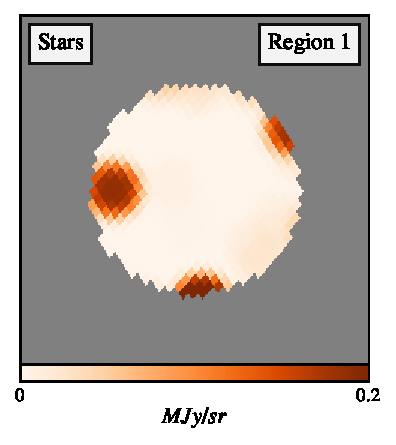
\includegraphics[width=0.24\textwidth]{figs/regions/stars_region_0.pdf}
  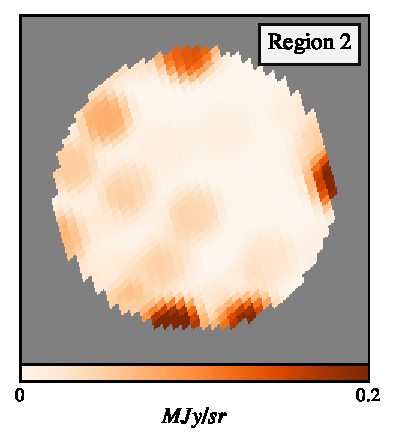
\includegraphics[width=0.24\textwidth]{figs/regions/stars_region_1.pdf}
    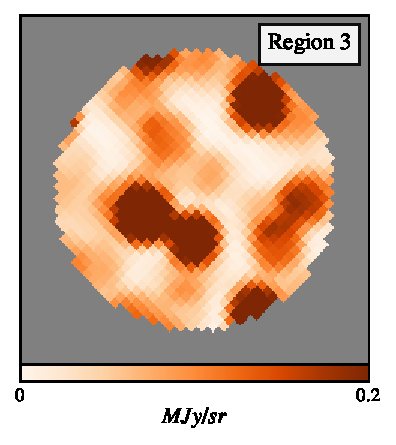
\includegraphics[width=0.24\textwidth]{figs/regions/stars_region_2.pdf}
      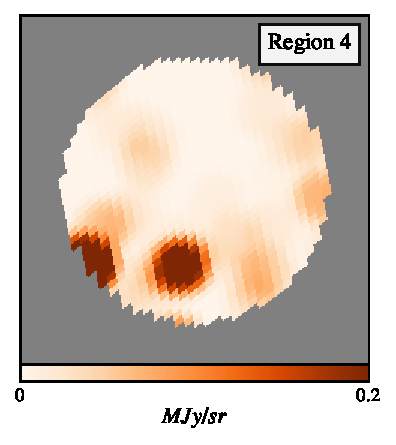
\includegraphics[width=0.24\textwidth]{figs/regions/stars_region_3.pdf}\\
        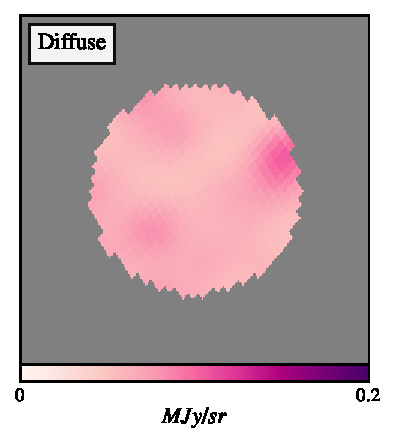
\includegraphics[width=0.24\textwidth]{figs/regions/diffuse_region_0.pdf}
  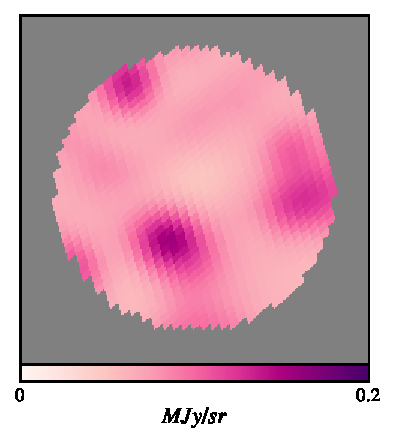
\includegraphics[width=0.24\textwidth]{figs/regions/diffuse_region_1.pdf}
    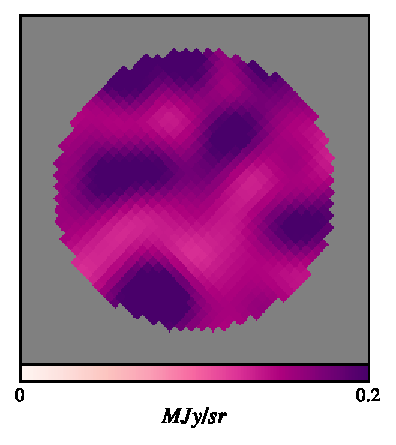
\includegraphics[width=0.24\textwidth]{figs/regions/diffuse_region_2.pdf}
      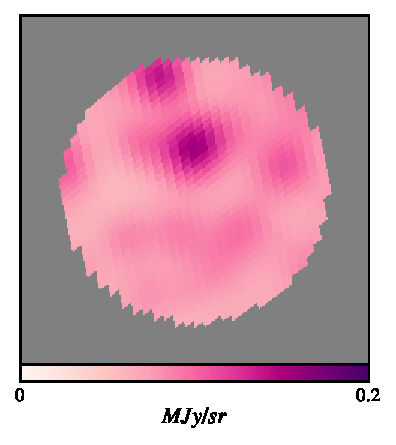
\includegraphics[width=0.24\textwidth]{figs/regions/diffuse_region_3.pdf}\\
        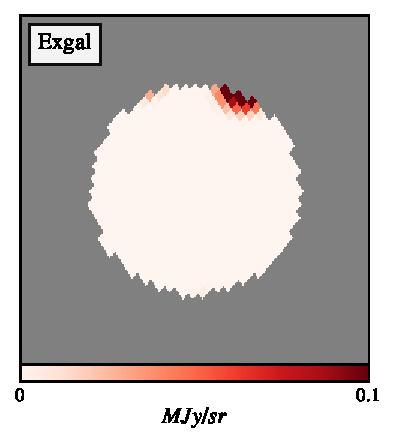
\includegraphics[width=0.24\textwidth]{figs/regions/exgal_region_0.pdf}
  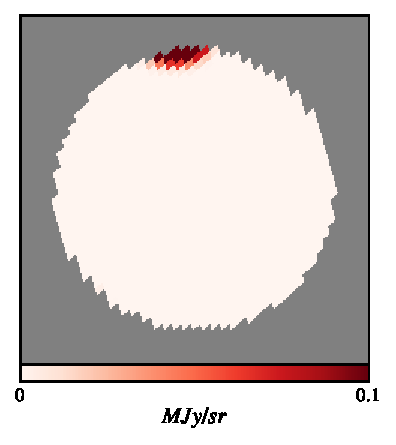
\includegraphics[width=0.24\textwidth]{figs/regions/exgal_region_1.pdf}
    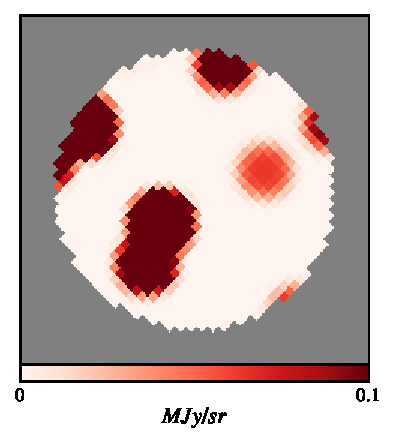
\includegraphics[width=0.24\textwidth]{figs/regions/exgal_region_2.pdf}
      \includegraphics[width=0.24\textwidth]{figs/regions/exgal_region_3.pdf}\\

  \caption{The four regions from \cite{DIRBE2mass}, shown from left to right. From top to bottom, we have the star emission, the diffuse template and the extragalactic sources. }
  \label{fig:regions}
\end{figure*}

The four regions are shown in Figure \ref{fig:regions}, left to right. We plot the stars, diffuse and extragalactic sources components for each region, showing the small scale structures. Differences in star classification between our analysis and \cite{DIRBE2mass} make it challenging to directly compare our amplitude estimates, but in general, the Cosmoglobe analysis predicts more star signal, especially in diffuse stars. \cite{DIRBE2mass} found that the bright stars were the brightest contribution to CIB foregrounds in DIRBE 01, whereas using a deeper star catalogue as we do in this work means that the unresolved diffuse stars actually end up being the dominant effect. In region 3, we also predict far more signal of all types than their analysis, driven by bright sources of all three classifications. By successfully modelling and removing more star emission, we are able to improve upon their limits on the CIB, as shown in \cite{CG02_02}. 

%\begin{figure}
%  \centering
%  \includegraphics[width=\columnwidth]{figs/mask_proc_calib.pdf}
%  \caption{Processing masks use in the analysis.}
%  \label{fig:masks}
%\end{figure}

Diffuse stars vs. point sources? 

Consistancy with WISE

Types of objects, classification?

Extinction? Finkbinder + schlagel

\subsection{Beam Estimation}

Another comparison that can be taken between this work and other analyses is an assessment of the averaged beam profile. DIRBE measured their beams from the 

We can also obtain an estimate of the beams directly from the data. For a given frequency map at a band i, we can approximate the full data model as 

\begin{equation}
M_i \approx \sum_{n=1}^{N} p_n \circledast B_i,
\label{eq:beammodel}
\end{equation}

where $M$ is the map, $p_n$ are the list of all pointsources and $B$ is the beam window function. Equation \ref{eq:beammodel} is obviously not true in general, but for bands where the sky is dominated by pointsources this approach is at least approximately correct. If we take the zodi-subtracted maps and mask out the regions in the galactic center where we have known residuals from other components, then we have 

\begin{equation}
m * M_i = \sum_{n=1}^{N} (m*p_n) \circledast B_i,
\label{eq:maskedbeam}
\end{equation}

where $m$ is now a mask which removes the regions in the galactic center. In bands 1-4, where the point sources are by far the brightest signal, this assumption is enough to produce an estimate of the beam function by simply taking the expression and converting to $a_{l,m}$s such that

\begin{equation}
M'_{alm} = s'_{alm} * B_i,
\label{eq:maskedbeam}
\end{equation}

where $M'$ is the masked map, and $s'$ is the masked sky, which is the sum of all the pointsources of equation \ref{eq:maskedbeam}. From here, it is a simple matter to divide the two quantities and convert to $c_l$s to extract the averaged beam window function $B_l$.

\begin{figure*}
  \centering
  \includegraphics[width=0.49\textwidth]{figs/stacking/beam_01.pdf}
  \includegraphics[width=0.49\textwidth]{figs/stacking/beam_02.pdf}\\
  \includegraphics[width=0.49\textwidth]{figs/stacking/beam_03.pdf}
  \includegraphics[width=0.49\textwidth]{figs/stacking/beam_04.pdf}\\

  \caption{Beam estimates from pointsources in the first 4 DIRBE bands.}
  \label{fig:beams}
\end{figure*}

Figure \ref{fig:beams} shows these window functions for bands 1-4, normalized to unity at $l=0$. 


\section{Conclusions}
\label{sec:conclusions}

Stars are a critical component of the infrared sky, which must be correctly modelled in order to avoid contaminating other components. 

Impact of star modelling

\subsection{Future Work}

Including the WISE data directly in the full run would be an important next step, and could potentially give enough extra information to constrain the star SEDs directly instead of pre-computing them. 




\begin{acknowledgements}
 The current work has received funding from the European
  Union’s Horizon 2020 research and innovation programme under grant
  agreement numbers 819478 (ERC; \textsc{Cosmoglobe}) and 772253 (ERC;
  \textsc{bits2cosmology}). Some of the results in this paper have been derived using the HEALPix \citep{healpix} package.
  We acknowledge the use of the Legacy Archive for Microwave Background Data
  Analysis (LAMBDA), part of the High Energy Astrophysics Science Archive Center
  (HEASARC). HEASARC/LAMBDA is a service of the Astrophysics Science Division at
  the NASA Goddard Space Flight Center.  
  
   This publication makes use of data products from the Wide-field Infrared Survey Explorer, which is a joint project of the University of California, Los Angeles, and the Jet Propulsion Laboratory/California Institute of Technology, and NEOWISE, which is a project of the Jet Propulsion Laboratory/California Institute of Technology. WISE and NEOWISE are funded by the National Aeronautics and Space Administration.
   
   This work has made use of data from the European Space Agency (ESA) mission
{\it Gaia} (\url{https://www.cosmos.esa.int/gaia}), processed by the {\it Gaia}
Data Processing and Analysis Consortium (DPAC,
\url{https://www.cosmos.esa.int/web/gaia/dpac/consortium}). Funding for the DPAC
has been provided by national institutions, in particular the institutions
participating in the {\it Gaia} Multilateral Agreement.
\end{acknowledgements}


%-------------------------------------------------------------
%                                       Table with references 
%-------------------------------------------------------------
%

\bibliographystyle{aa}
\bibliography{references, ../../common/CG_bibliography}
\end{document}
%%%% End of aa.dem
